\chapterimage{ChapterImageLaboratory.png} % Chapter heading image

\chapter{Water Quality \& Laboratory Procedures}





% Please add the following required packages to your document preamble:
% \usepackage[normalem]{ulem}
% \useunder{\uline}{\ul}{}
% Please add the following required packages to your document preamble:
% \usepackage[normalem]{ulem}
% \useunder{\uline}{\ul}{}
\begin{table}[H]
\begin{tabular}{| m{1cm} | m{15cm} |}
\hline
\multicolumn{2}{|l|}{\textbf{Expected   Range of Knowledge for Water Properties and Sources}}                                                                          \\ \hline
\multicolumn{2}{|l|}{\textit{Water   Distribution System Operator License Exams}}                                                                                      \\ \hline

D1 & Ability to read   a graduated cylinder                                                            \\ \hline
D1 & Ability to interpret   coliform test results                                                      \\ \hline
D1 & Knowledge of coliform   analysis methods                                                          \\ \hline
D1 & Knowledge of coliform   bacteria types                                                            \\ \hline
D1 & Knowledge of the   definition of pathogenic organisms                                             \\ \hline
D1 & Knowledge of holding   times (e.g. preservatives)                                                 \\ \hline
D1 & Knowledge of water   sampling techniques for bacteriological, organic, and inorganic constituents \\ \hline
D2 & Knowledge of the use   of coliform as a surrogate                                                 \\ \hline
D2 & Ability to   distinguish between presumptive and confirmed results                                \\ \hline
D2 & Knowledge of nitrate   formation in a distribution system                                         \\ \hline
D2 & Knowledge of   potential waterborne diseases                                                      \\ \hline
D2 & Knowledge of the   effects of abnormal pH levels in a distribution system                         \\ \hline
D2 & Knowledge of the   effects of hardness in a distribution system                                   \\ \hline
D2 & Knowledge of the   effects of heterotrophic bacteria in a distribution system                     \\ \hline
D3 & Knowledge of the   galvanic series                                                                \\ \hline
D3 & Knowledge of the   Langelier Index                                                                \\ \hline
D3 & Knowledge of common   inorganic contaminant compounds pH, Conductivity, Hardness, and Turbidity   \\ \hline
D3 & Knowledge of common   organic contaminant compounds                                               \\ \hline
D3 & Knowledge of sources   of inorganic contaminants in a distribution system                         \\ \hline
D3 & Knowledge of sources   of organic contaminants in a distribution system                           \\ \hline
D4 & Ability to interpret a Langelier Index                                                            \\ \hline

\end{tabular}
\end{table}


\newpage



\begin{table}[H]
\begin{tabular}{| m{1cm} |m{15cm} |}
\hline
\multicolumn{2}{|l|}{\textbf{Expected   Range of Knowledge for Water Properties and Sources}}                                                                      \\ \hline
\multicolumn{2}{|l|}{\textit{Water   Treatment Operator License Exams}}                                                                  \\ \hline
T1 & Ability to recognize   abnormal chemical characteristics of water                                 \\ \hline
T1 & Ability to recognize   abnormal odors or colors                                                   \\ \hline
T1 & Knowledge of   chemicals that contribute alkalinity and hardness to water                         \\ \hline
T1 & Knowledge of common   chemical and microbial contaminants in raw water                            \\ \hline
T1 & Knowledge of problems   caused by hard water                                                      \\ \hline
T1 & Knowledge of the   chemical components of groundwater and surface water                           \\ \hline
T1 & Ability to interpret   turbidity information                                                      \\ \hline
T1 & Knowledge of   turbidity causing matter                                                           \\ \hline
T1 & Knowledge of   chemicals that contribute hardness to water                                        \\ \hline
T1 & Ability to recognize   corrosion problems                                                         \\ \hline
T1 & Knowledge of pH   adjustment procedures                                                           \\ \hline
T1 & Knowledge of   corrosion causes                                                                   \\ \hline
T1 & Knowledge of abnormal   taste and odors                                                           \\ \hline
T1 & Knowledge of   chemicals that contribute taste and odor                                           \\ \hline
T1 & Knowledge of taste   and odor treatment processes                                                 \\ \hline
T1 & Ability to recognize   an iron and manganese problem                                              \\ \hline
T1 & Knowledge of health   effects of lead and copper                                                  \\ \hline
T1 & Knowledge of adverse   health effects caused by common contaminants                               \\ \hline
T1 & Ability to collect a   water sample                                                               \\ \hline
T1 & Ability to determine   a proper sampling site                                                     \\ \hline
T1 & Ability to follow   chain of custody                                                              \\ \hline
T1 & Knowledge of   appropriate sample containers and sample sizes                                     \\ \hline
T1 & Knowledge of maximum   holding times                                                              \\ \hline
T1 & Knowledge of proper   sampling and preservation techniques                                        \\ \hline
T1 & Knowledge of well   sampling techniques                                                           \\ \hline
T1 & Knowledge of chemical   hazards                                                                   \\ \hline
T1 & Ability to analyze a   water sample for free and total chlorine                                   \\ \hline
T1 & Ability to read and   interpret a colorimeter                                                     \\ \hline
T1 & Knowledge of approved   analytical procedures for chlorine analysis                               \\ \hline
T1 & Ability to read and   interpret a pH meter                                                        \\ \hline
T1 & Knowledge of acids   and bases                                                                    \\ \hline
T1 & Knowledge of   acceptable water pH range                                                          \\ \hline
T1 & Knowledge of   chemicals that affect the pH of water                                              \\ \hline
T1 & Knowledge of the   effects of pH on water quality                                                 \\ \hline
T1 & Knowledge of the pH   scale                                                                       \\ \hline
T1 & Ability to analyze a   water sample for pH                                                        \\ \hline
T1 & Ability to analyze a   water sample for turbidity                                                 \\ \hline
T1 & Ability to read and   interpret a turbidimeter                                                    \\ \hline
T1 & Knowledge of the   Nephelometric Turbidity Unit (NTU) scale                                       \\ \hline
T1 & Knowledge of   turbidimeter instrumentation                                                       \\ \hline
T1 & Knowledge of   turbidity level requirements                                                       \\ \hline
T1 & Ability to identify   an objectionable taste or odor in water                                     \\ \hline
T1 & Knowledge of   chemicals that contribute taste and odor to water                                  \\ \hline
T1 & Knowledge of the   presence/absence test method                                                   \\ \hline
T1 & Knowledge of approved   analytical procedures for coliform analysis                               \\ \hline
T1 & Knowledge of common   microbial contaminants in raw water                                         \\ \hline
T1 & Ability to interpret   water quality characteristics (hardness, turbidity, pH )                   \\ \hline
\end{tabular}
\end{table}
\newpage



\begin{table}[H]
\begin{tabular}{| m{1cm} |m{15cm} |}
\hline
\multicolumn{2}{|l|}{\textbf{Expected   Range of Knowledge for Water Properties and Sources}}                                                                      \\ \hline
\multicolumn{2}{|l|}{\textit{Water   Treatment System Operator License Exams (Continued)}}                                                                  \\ \hline
T1 & Ability to recognize   abnormal chemical characteristics of water                                 \\ \hline
T2 & Ability to prepare   and calibrate turbidimeter with Primary Standard (Formazin)                  \\ \hline
T2 & Ability to analyze a   water sample for water hardness                                            \\ \hline
T2 & Ability to recognize   abnormal colors in water                                                   \\ \hline
T2 & Knowledge of   Heterotrophic Plate Count (HPC)                                                    \\ \hline
T3 & Knowledge of the   Langelier Index                                                                \\ \hline
T3 & Knowledge of   corrosion control chemical reactions                                               \\ \hline
T3 & Knowledge of iron and   manganese oxidation chemistry                                             \\ \hline
T3 & Knowledge of   chemicals that contribute alkalinity to water                                      \\ \hline
T3 & Ability to use a   titrator                                                                       \\ \hline
T3 & Ability to recognize   a titration endpoint                                                       \\ \hline
T3 & Knowledge of abnormal   alkalinity levels                                                         \\ \hline
T3 & Ability to analyze a   water sample for specific conductance                                      \\ \hline
T3 & Ability to read and   interpret a specific conductance meter                                      \\ \hline
T3 & Knowledge of abnormal   color levels                                                              \\ \hline
T3 & Ability to   distinguish between presumptive and confirmed coliform results                       \\ \hline
T3 & Knowledge of the   multiple tube fermentation method                                              \\ \hline
T3 & Knowledge of the   membrane filtration method                                                     \\ \hline
T4 & Knowledge of the   health effects of fluoride                                                     \\ \hline
T4 & Ability to calculate   a TDS value from a specific conductance reading                            \\ \hline
T4 & Knowledge of EC/TDS   ratio                                                                       \\ \hline
T4 & Ability to calibrate   a specific conductance meter                                               \\ \hline
T4 & Ability to operate an   Ion Specific Electrode (ISE)                                              \\ \hline
T4 & Knowledge of optimal   fluoride level range                                                       \\ \hline
T4 & Knowledge of color   analysis scale                                                               \\ \hline
T4 & Knowledge of true and   apparent color                                                            \\ \hline
T4 & Knowledge of odor   analysis protocol                                                             \\ \hline
\end{tabular}
\end{table}

\newpage
Water occurring in nature will have other elements dissolved or suspended in it. A "contaminant" is a physical, chemical, biological, or radiological substance or matter, in water.  The type and amount of these contaminants will affect the property and safety of that water, if it is to be used as drinking water.  Some drinking water contaminants may be harmful if consumed at certain levels in drinking water while others may be harmless. The presence of contaminants does not necessarily indicate that the water poses a health risk.\\

Contaminants in drinking water can be broadly categorized as:
\begin{itemize}
\item \ul{Chemical contaminants} \index{Chemical contaminants} which may be naturally occurring or man-made elements or compounds. Examples of chemical contaminants include nitrogen, bleach, salts, pesticides, metals, and human or animal drugs.
\item \ul{Biological contaminants} \index{Biological contaminants} which are also refered as micorbes or microbiological contaminants which include bacteria, viruses, protozoa and parasites.
organisms
\item \ul{Radiological contaminants} \index{Radiological contaminants} which are chemical compounds or elements which contain unstable atoms that emit ionizing radiation.  Example of radiological contaminants include, cesium, plutonium and uranium.
\end{itemize}

\section{Organics}\index{Organics}
\begin{itemize}
\item Organics – are carbon based material can originate from lifeforms or can be man-made.
\item Only few carbon compounds such as carbonates, cyanides are not classified as organic.
\item In water they originate from decaying plant and animal life and wastes.
\item Amount present in natural waters is usually low. 
\item Many organic compounds are soluble in water, and surface waters are more prone to contamination by natural organic compounds than are groundwaters.
\item Synthetic organic compounds, such as polychlorinated biphenyls (PCBs), dioxin, and dichlorodiphenyl-trichloroethane (DDT), all of which are toxic, often persist and accumulate because they do not readily break down in natural ecosystems. 
\item Many of the organic compounds found in water are known to cause cancer and birth defects in people. 
\item Organic matter in water is responsible for:
\begin{itemize}
\item Color formation
\item Taste and odor problems
\item Oxygen depletion in streams
\item Interference with water treatment processes, and
\item Formation of halogenated compounds when chlorine is added to disinfect water.
\end{itemize}
\item The quantity of oxygen-consuming organics in water is usually determined by measuring its biochemical oxygen demand (BOD)\index{Organics!Quantification!Biochemical oxygen demand (BOD)}
\item BOD is the amount of dissolved oxygen required by aerobic decomposers to break down the organic materials in a given volume of water over a 5-day incubation period at 20\degree{C} (68\degree{F}).
\end{itemize}

\section{Inorganics} \index{Inorganics}
Inorganic elements do not contain carbon and are not derived from living material. The inorganics include metals, acids, bases, salts, oxides, sulfate, phosphates, etc.
\subsection{Metals}\index{Metals}
\begin{itemize}
\item Iron and Manganese:\\
\begin{itemize}
\item Although iron and manganese are most commonly found metals in groundwaters, surfacewaters may also contain significant amounts at times. 
\item Non-pathogenic bacteria feed on iron and manganese in water to form red-brown (iron) or black-brown (manganese) slime which accumulates on spouts and inside toilet tanks.
\item Iron is a secondary or aesthetic contaminant and dissolved iron gives water a disagreeable metallic taste.
\item An iron concentration of 0.3 mg/l can cause water to turn a reddish brown color and leave reddish brown stains which are very hard to remove.
\end{itemize}
\item Calcium and magnesium: \index{Calcium} \index{Magnesium}\\
\begin{itemize}
\item The metals most often found in the highest concentrations in natural waters are calcium and magnesium. These are usually associated with a carbonate anion and come from the dissolution of limestone rock.
\item Calcium and magnesium are nontoxic and normally absorbed by living organisms more readily than the other metals; therefore, if the water is hard, the toxicity of a given concentration of a toxic metal is reduced. 
\item Conversely, in soft, acidic water, the same concentrations of metals may be more toxic. 
\item In natural water systems, other nontoxic metals are generally found in very small quantities. Most of these will cause taste problems well before they reach toxic levels.
\end{itemize}
\item Heavy metals:\\
\begin{itemize}
\item Even in small quantities, toxic metals including: arsenic, barium, cadmium,chromium, lead, mercury, and silver in drinking water are harmful to humans and other organisms. Arsenic, cadmium, lead and mercury, all cumulative toxins, are particularly hazardous.These particular metals are concentrated by the food chain, thereby posing the greatest danger to organisms near the top of the chain.
\end{itemize}
\end{itemize}
\begin{figure}[]
\begin{center}
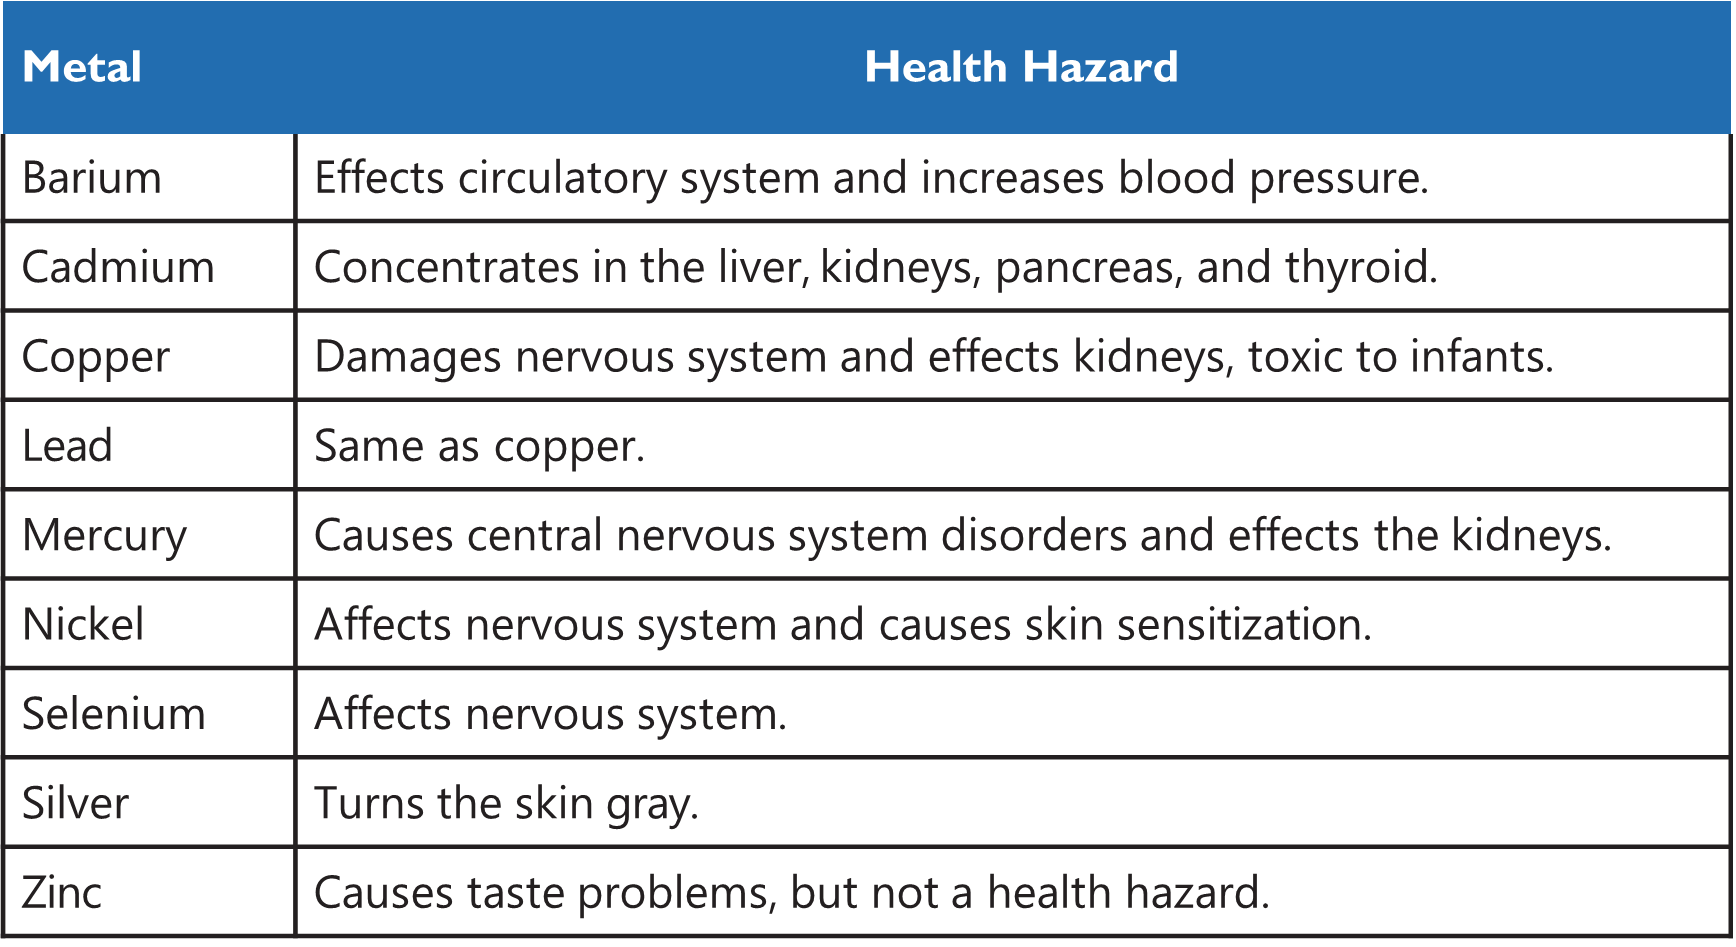
\includegraphics[scale=0.75]{MetalHealthHazard}
\caption{Metals in drinking water - health hazards}\index{Metals!Health hazards}
\end{center}
\end{figure}
\subsection{Salts}\index{Salts}
\begin{itemize}
\item A salt is formed when a metal ion (cation - because it has a positive charge) combines with a nonmetal ion (anion - because it has a negative charge). For instance, when a metal like sodium combines with a non-metal ion like chloride to form sodium chloride, NaCl, or table salt. \index{Anion} \index{Cation}

\item Common metal anions and cations that combine to form salts which are commonly found in drinking water supplies or used in Water treatment are listed in the table below.
\end{itemize}

\begin{table}[h!]    
\begin{center}
     \begin{tabular}{ | m{5cm}  m{5cm} |}
     \hline
           \multicolumn{1}{|c}{} & \multicolumn{1}{c|}{} \\
      \multicolumn{1}{|c}{\textbf{METAL ION (CATION)}} & \multicolumn{1}{c|}{\textbf{NON-METAL ION (ANION)}} \\
            \multicolumn{1}{|c}{} & \multicolumn{1}{c|}{}\\
      Calcium - Ca$^{+2}$ & Carbonate - CO$_3^{\enspace -1}$\\
      Magnesium - Mg$^{+2}$ & Bicarbonate - HCO$_3^{\enspace -1}$\\
      Manganese - Mn$^{+2}$ & Hydroxide - OH$^{-1}$\\
      Iron - Fe$^{+2/+3}$ & Sulfate - SO$_4^{\enspace -2}$\\
      Aluminum - Al$^{+3}$ & Chloride - Cl$^{-1}$\\
      Sodium - Na$^{+1}$ & \\
      Copper - Cu$^{+2/+3}$ & \\
          \hline
                    \end{tabular}
     \caption{Salts constituents}
     \label{Salts constituents}\index{Salts constituents}
     
\end{center}
     \end{table}

\begin{table}[h!]    
\begin{center}
     \begin{tabular}{ | m{5cm}  m{4cm}  m{4cm} |}
     \hline
           \multicolumn{1}{|c}{} & \multicolumn{1}{c}{} & \multicolumn{1}{c|}{}\\
      \multicolumn{1}{|c}{\textbf{CHEMICAL NAME}} & \multicolumn{1}{c}{\textbf{FORMULA}} & \multicolumn{1}{c|}{\textbf{COMMON NAME}}\\
            \multicolumn{1}{|c}{} & \multicolumn{1}{c}{} & \multicolumn{1}{c|}{}\\
      Aluminum sulfate & Al$_2$(SO$_4$)$_3$ & Alum\\
      Calcium oxide & Ca$ $O$ $ $ $ & Quicklime\\
      Calcium hydroxide & Ca$ $(OH$ $)$_2$ & Slaked/hydrated lime\\
      Calcium carbonate & Ca$ $CO$_3$ $ $ & Limestone\\
      Calcium hydroxide & Ca$ $(OH$ $)$_2$ & Slaked/hydrated lime\\
      Magnesium carbonate & Mg$ $(CO$_3$)$_2$ & \\
      Magnesium bicarbonate & Mg$ $(HCO$_3$)$_2$ & \\
      Sodium hydroxide & Na$ $OH$ $ $ $ & Caustic soda\\
      Sodium carbonate & Na$_2$CO$_3$ $ $ & Soda ash\\
      Ferrous sulfate & Fe$ $SO$_4$ $ $ & Copperas \\
      Ferric chloride & Fe$ $Cl$_3$ $ $ & \\
      Ferrous chloride & Fe$ $Cl$_2$ $ $ & \\
      Copper sulfate & Cu$ $SO$_4$ $ $ &\\

          \hline
                    \end{tabular}
     \caption{Salts found in water and/or used in water treatment}
     \label{Salts found in water and/or used in water treatment}\index{Salts found in water and/or used in water treatment}
     
\end{center}
     \end{table}

\subsection{Nutrients}\index{Nutrients}
\begin{itemize}
\item Plant nutrients - nitrogen and phosphorous\index{Nutrients!Nitrogen and phosphorous}, present in water promote growth of plant and algal matter in the receiving waters causing destruction of the normal aquatic life mainly due to oxygen depletion - eutrophication\index{Eutrophication}.
\item Major sources of nitrogen include runoff from animal feedlots, fertilizer runoff from agricultural lands, municipal wastewater discharges, and certain bacteria and blue-green algae than can obtain nitrogen directly from the atmosphere In addition,certain forms of acid rain can also contribute nitrogen to surface waters. Nitrogen in water is commonly found in the form of nitrate (NO$_3^{\enspace-}$) \index{Nitrates}
\item Nitrate in drinking water can lead to serious problems, specifically nitrate poisoning which can lead to death. Bacteria commonly found in the intestinal tract of infants can convert nitrate to highly toxic nitrites (NO$_2^{\enspace-}$). Nitrite can replace oxygen in the bloodstream and result in oxygen starvation, which causes a bluish discoloration of the infant known as infant methemoglobinemia or blue-baby syndrome \index{Infant methemoglobinemia or blue-baby syndrome}.  High nitrate levels may also affect the oxygen-carrying ability of the blood of pregnant women.
\item Nitrifying bacteria present in biological slime in the distribution system convert ammonia and other nitrogen compounds into nitrite (NO$_2$ $^-$) and then nitrate (NO$_3^{\enspace-}$).  This process is called nitrification. \index{Nitrification}
\item Major sources of phosphorous include phosphates in detergents, fertilizers and feedlot runoff, as well as municipal wastewater discharges.
\item Phosphate is added as part of the water treatment for corrosion control and for improving taste and odor by sequestering iron and magnesium.

\end{itemize}

\section{Trace constituents} \index{Trace constituents}
\begin{itemize}
\item Trace Constituents are chemicals found in extremely low concentrations.
\item Trace constituents include:
\begin{itemize}
\item B - Boron
\item Miscellaneous metals
\item Hormones
\item EDCs - Endocrine-disrupting compounds are synthetic and natural compounds that mimic, block, stimulate, or inhibit natural hormones in the endocrine systems of animals, including humans. The origins include pesticides, pharmaceutically active chemicals (PhACs), personal care products (PCPs), herbicides, industrial chemicals, and disinfection byproducts (DBPs).
\item PCPs - Personal Care Products are products such as shampoo, hair conditioner, deodorants, and body lotion.
\item Pharmaceuticals - aspirin, ibuprofen, caffeine, etc.
\item CECs - Constituents of Emerging Concern is a general term applied to constituents that have relatively recently become known as a potential concern and likely have little to no information available to fully comprehend and establish safe and realistic standards, such as PFAS/PFOA \index{PFAS/PFOA}.
\index{Trace constituents!Boron, hormones, EDCs, PCPs, CECs, PFAS/PFOA}
\end{itemize}
\end{itemize}

\section{Radionuclides}\index{Radionuclides}
\begin{itemize}
\item Radioactive materials, also called radionuclides, are both naturally occurring and human-made.

\item Radionuclides such as radium, radon and uranium can get into groundwater and surface waters from natural sources and also potentially from human sources such as active nuclear power plants or other facilities that make or use radioactive substances.

\item When radionuclides break down (decay), they emit radioactive particles such as alpha-particles, beta-particles and gamma-rays radiation which could present a risk to human health.

\item Most water systems have no detectable radionuclide activities, some areas of the United
States have significantly higher levels than the national averages.

\item People who are exposed to relatively high levels of radionuclides in drinking water for long periods may develop serious health problems, such as cancer, anemia, osteoporosis, cataracts, bone growths, kidney disease, liver disease and impaired immune systems.

\item The health risks associated with radionuclides are normally small compared with the risks from microorganisms and chemicals that may be present in drinking-water. 

\item The amount of radionuclides in drinking water is quantified and regulated under the EPA's Radionuclide Rule, by standards based upon both, the radioactivity levels as measured by the radiation of alpha and beta particles and the amount of commonly found radioactive elements - radium and uranium, quantified in terms of their radioactivity.
\item For drinking water, radiation/radioactivity levels is measured as pCi/L (picocuries per liter)\index{Radionuclides!Measurement!picocuries per liter (pCi/L)}
\end{itemize}



\section{Microbial contaminants}\index{Microbial contaminants}
\begin{itemize}
\item Many types of \textbf{pathogenic} - disease-causing germs can be found in contaminated drinking water, including bacteria, viruses and parasites.

\item Common virus in drinking water \index{Pathogens!Viruses} source and their associated diseases include:
\begin{itemize}
\item Adenoviruses - tonsillitis, conjunctivitis, the common cold and other illnesses. 
\item Reoviruses - colds, flu, diarrhea, chicken pox, measles and mumps.
\item polioviruses - polio
\item hepatitis A virus
\end{itemize}

\item Some of the water borne pathogenic bacteria \index{Pathogens!Bacteria} and their associated disease include:
\begin{itemize}
\item Salmonella typhi - Typhoid fever
\item Vibrio cholerae - cholera
\item Yersinia enterocolitica - gastroenteritis
\end{itemize}

\item Common intestinal parasites and their associated disease include \index{Pathogens!Parasites}:
\begin{itemize}
\item Entamoeba histolytica - Amoebic Dysentery.
\item Giardial lamblia (Giardiasis) \index{Pathogens!Parasites!Giardia}.
\item Ascaris lumbricoides (Giant Roundworm).
\item Cryptosporidium (Cryptosporidiosis) \index{Pathogens!Parasites!Cryptosporidium}.
\end{itemize}


\end{itemize}
 



\section{Physicochemical tests} \index{Physicochemical tests}

\begin{itemize}
\item The aesthetic quality \index{Aesthetic quality} aspects of drinking water include: taste, odor, color, turbidity, hardness, and temperature.
\item The aesthetics are generally not health-related. However, consumers can easily detect them, so they can have significant effects on perceptions of water quality and acceptability.
\item These attributes are the source of most complaints to water suppliers and frequently lead consumers to choose home treatment or bottled water.
\end{itemize}
\subsection{Turbidity}\index{Turbidity}
\begin{itemize}
\item Measures cloudiness of water due to suspended particles.
\item Higher turbidity levels are often associated with higher levels of disease-causing microorganisms.
\item Turbidity affects both the acceptability of water to consumers
\item Harmful pollutants such as heavy metals and pesticides are easily absorbed by suspended solids
\item Turbidity affects disinfection as suspended particles in water act as a protective shield for micro-organisms and provide an excellent substrate for bacteria growth.  Higher disinfection doses or contact times are required to ensure adequate treatment.
\item Suspended solids represent a risk for the main water distribution systems, pumps and other equipment where tend to deposit and block pipes and nozzles.
\item Turbidity is an optical measurement of water's ability to scatter and absorb light rather than transmit it in straight lines.  It is commonly measured in the unit of Nephelometric Turbidity Units (\textbf{NTU}). \index{Nephelometric Turbidity Units (NTU)}
\item "Crystal-clear” water has a turbidity of <1 NTU; at 4 NTU and above, water becomes visibly cloudy at 25 NTU it is murky.
\item An average person is able to see turbidity with the naked eye at NTU level of 5 and above.
\item Sources of turbidity:
\begin{enumerate}
\item In source water, turbidity can be attributed to:
\begin{itemize}
\item Inorganic particles released by weathering of rocks, soils and clays
\item Human, livestock and industrial wastes
\item Biological growth (e.g. algae, zooplankton and cyanobacteria) in source waters
\item Natural organic matter including decomposing plant material
\end{itemize}
\item Introduction of turbidity during treatment can be due to:
\begin{itemize}
\item Poor control of treatment chemical dosing (e.g. coagulants, settling aids and pH adjustment chemicals)
\item Precipitates from insoluble components of treatment chemicals, or formed during processes such as pH correction
\item Oxidation products of natural chemicals such as arsenic, iron and manganese
\end{itemize}
\item Turbidity can also be introduced in the distribution system by: \index{Turbidity}
\begin{itemize} 
\item Intrusion of soils and sewage through mains breaks
\item External contamination from backflow or cross connections
\item Resuspension of accumulated silts and sediments, or detachment of corrosion chemicals and scales and detachment of biofilms
\end{itemize}
\end{enumerate}
\item Formazin \index{Formazin} - a chemical, is used for preparing solutions of known turbidities.
\end{itemize}

\subsection{Color}\index{Color}
\begin{itemize}
\item Color may affect the turbidity value but is distinct from turbidity as color is due to organic material that has dissolved into solution, while turbidity consists of tiny particles suspended in the water column.
\end{itemize}

\subsection{Taste and odor}\index{Taste and odor}
\begin{itemize}
\item Odor and taste are useful indicators of water quality even though odor and taste-free water is not necessarily safe to drink nor water with some odors or taste is necessarily harmful.
\item Taste and odors are often grouped with odor because of their common origin factors. 
\item The cause of taste and odor issues can be from water fixtures, plumbing materials, water heaters, water treatment, pressure tanks and/or the source (the well).
\item Taste and odors are generally attributed to the presence of organic and some inorganic chemicals which come from the decaying organic matter, runoffs, industrial wastes, and municipal sewage discharges. 
\item Geosmin and methyl-isoborneol (MIB) are often the cause of earthy-musty odors occurring in fall due to the turnover of lakes and reservoirs.  They are produced by bacteria, particularly actinomycetes and cause odor issues at a very low concentrations.
\item In the groundwater, the tastes and odors can be due to iron, manganese, and hydrogen sulfide (H$_2$S).
\item Often, identifying the exact origin of taste and odor is usually very expensive and often impossible, and removal of the causative substance is even harder.
\item Current methods of measuring taste and odor are still fairly subjective.  Standards related to odor and taste: Chloride, Copper, Foaming Agents, Iron, Manganese pH, Sulfate, Threshold Odor Number (\textbf{TON})\index{Threshold odor number (TON)} which is the greatest dilution of a sample with odor-free water that still yields a just-detectable odor.
\end{itemize}

\subsection{Temperature}\index{Temperature}
\begin{itemize}
\item Temperature affects the solubility of oxygen in water, the rate of bacterial activity, and the rate at which gases are transferred to and from the water.
\item Cool water is generally more palatable than warm water, and temperature will have an impact on the acceptability of a number of other inorganic constituents and chemical contaminants that may affect taste. 
\item High water temperature enhances the growth of microorganisms and may increase problems related to taste, odor, color and corrosion.
\item Water temperature determines, in part, how efficiently certain water treatment processes operate. For example, temperature has an effect on the rate at which chemicals dissolve and react. When water is cold, more chemicals are required for efficient coagulation and flocculation to take place. When water temperature is high, the result may be a higher chlorine demand because of the increased reactivity, as well as an increased level of algae and other organic matter in raw water.
\item Heat is added to surface and groundwater from natural and man-made sources.  Surface waters in particular  are potentially subject to great temperature variations. 
\item Other sources of increased temperatures in running water result from forest clearing and return of irrigation flows to a body of running water.
\end{itemize}

\subsection{Total dissolved solids}\index{Total dissolved solids}
\begin{itemize}
\item Total dissolved solids (\textbf{TDS}) is a part of total solids (\textbf{TS}) in water and are the material remaining in water after filtration.
\item Components of water TDS include:
\begin{itemize}
\item Minerals from rocks and soil as water passes over and through them.
\item Pesticides and herbicides from agricultural runoff
\item Lead and copper from plumbing pipes
\item Chemicals added during water treatment
\item Human and animal wastes
\item Biological decay products
\end{itemize}
\item Water has an equilibrium state with respect to dissolved portion; thus, if water is under saturated, it will aggressively dissolve materials it comes into contact with. Because of this problem, certain soluble substances, typically calcium and magnesium based substances are added post water treatment to minimize its corrosivity effects in the distribution system.
\item Dissolved solids can be removed from water by distillation, electro-dialysis, reverse osmosis, or ion exchange.
\item TDS is measured in mg/L or ppm.  
\item As water will conduct electricity due to the presence of dissolved inorganic ions, higher the concentration of these ions, the higher is the conductivity. Thus, specific conductance \index{Specific conductance} - conductivity measurement, provides a good estimate of the water's TDS.
\item The terms “specific conductance,” “specific electrical conductance,” and
“electrical conductivity” are used interchangeably and its unit of measurement is in Siemens per centimeter (S/cm) or mhos per centimeter (mhos/cm) \index{mhos per centimeter (mhos/cm)} \index{Siemens per centimeter (S/cm)}.
\item The TDS concentration is considered a Secondary Drinking Water Standard, which means that it is not a health hazard.
\item EPA has established a Secondary Drinking Water Standard of a maximum concentration of 500 mg/l of TDS \index{Total dissolved solids!Secondary standard}in drinking water and  recommends treatment when TDS concentrations exceed 500 mg/L, or 500 parts per million (ppm). 
\end{itemize} 

\subsection{pH}\index{pH}	
			pH is a measure of the hydrogen ion (H$^+$) content or the acidity or basicity of a solution.  pH impacts the chemical and microbiological elements of water treatment processes and thus pH measurement and control is critical.
			\begin{itemize}
				\item Pure water dissociates into equal concentration of hydrogen ions and hydroxide ions:\\ 
				      $H_2O \rightarrow H^+ + OH^-$.
				\item The H$^+$ are responsible for acidic properties and the OH$^-$ ions for the basic properties.  
				\item pH is the inverse of H$^+$ concentration; pH increases when the concentration of H$^+$ decreases relative to the concentration of OH-. 
				\item pH scale ranges from 0 – 14. When the concentration of both H$^+$ and OH$^-$ are equal, as in pure water, it is considered neutral and its pH is 7.0.  \item If the pH of a sample solution is below 7.0, the sample is termed acidic and is alkaline or basic if its pH is above 7.0. 
				\item Each change of 1 pH unit represents a 10 fold change in concentration.  For example, a sample with a pH of 2.0 is 1000 times more acidic than a sample with a pH of 5.0.
				
				\item The affects of drinking water pH include:
				\begin{itemize}
				\item Taste and odor impacts.
				\item Solubility and biological availability of chemical constituents such as nutrients - phosphorus, nitrogen, and carbon.
				\item Solubility and toxicity of heavy metals.  Metals tend to be more toxic at lower pH because they are more soluble.
				\end{itemize} 
				\item pH is measured by an electrode that is sensitive only to H$^+$ or using a pH strip which is essentially an adsorbent paper which is pre-impregnated with chemicals which change color under different H$^+$ concentrations.
						
\item \index{pH!pH measurement}It is important to measure pH at the same time as chlorine residual since the efficacy of disinfection with chlorine is highly pH-dependent; where the pH exceeds 8.0, disinfection is less effective. To check that the pH is in the optimal range for disinfection with chlorine (less than 8.0), simple tests may be conducted in the field using comparators such as that used for chlorine residual. With some chlorine comparators, it is possible to measure pH and chlorine residual simultaneously.

\item Alternatively, portable pH electrodes and meters are available. If these are used in the laboratory, they must be calibrated against fresh pH standards at least daily; for field use, they should be calibrated immediately before each test. Results may be inaccurate if the water has a low buffering capacity.
\end{itemize}

\subsection{Alkalinity}\index{Alkalinity}
\begin{itemize}
\item Alkalinity is a measure of the ability of water to neutralize acid, or an expression of its buffering capacity.
\item Constituents of alkalinity are: Bicarbonate – HCO$_3$, Carbonate - CO$_3$ , Hydroxide - OH$^-$
\item Measured in equivalent of mg/L CaCO$_3$
\item Alkalinity levels can be classified as:
\begin{itemize}
\item Low Alkalinity - < 20 mg CaCO$_3$/L
\item Moderate Alkalinity - 20 to 160 mg CaCO$_3$/L
\item High Alkalinity - > 160 mg CaCO$_3$/L
\end{itemize}
\item High alkalinity indicates the scaling (deposit forming) potential and salty taste
\item Low alkalinity implies undersaturation of water (absence of dissolved content) and thus would exhibit higher corrosion potential - tendency to dissolve metals.
\item Alkalinity originates naturally as water moves through rocks dissolving minerals.
\item Alkalinity is important for fish and aquatic life because it protects or buffers against rapid pH changes. In addition, alkalinity levels affect the efficiency of certain water treatment processes, especially the coagulation process.
\end{itemize}


\subsection{Hardness}\index{Hardness}
\begin{itemize}
\item Hardness is due to the presence of multivalent metal ions, which come from minerals dissolved in water.  The dissolution of these minerals is aided by the carbonic acid formed by the dissolution of naturally occurring carbon dioxide in water. 
\item Domestic use of hard water is marked by lack of foam formation with soap solutions due to the formation of a white precipitate (soap scum) instead of producing lather and formation of noticeable limescale in kettles and water heaters.
\item Calcium (Ca) and Magnesium (Mg) \index{Calcium} \index{Magnesium} are the two metals that dissolve the most easily in water. They are considered to be the main cause of hardness.
\item Hardness causing compounds are broken into two groups:\\
\begin{itemize}
\item \ul{Carbonate hardness or temporary hardness} \index{Carbonate hardness or temporary hardness}which is the hardness that can be removed by boiling water.
\begin{itemize}
\item Carbonate hardness is formed when calcium or magnesium combines with a form of alkalinity (carbonate, bicarbonates, or hydroxides.) 
\end{itemize}
\item \ul{Non-carbonate hardness} \index{Hardness!Carbonate hardness} cannot be removed by boiling water.
\begin{itemize}
\item Non-carbonate hardness \index{Hardness!Non-carbonate hardness}is formed when calcium and magnesium combine with anything other than alkalinity. Chlorides and sulfates are the two most common forms of non-carbonate hardness.
\end{itemize}
\end{itemize}
\item Hard water when used in industrial applications forms deposits - scale composed mainly of calcium carbonate (CaCO$_3$), magnesium hydroxide (Mg(OH)$_2$), and calcium sulfate (CaSO$_4$)on the inside surfaces of pipes and heat exchangers. The scale formed restricts the flow of water, heat transfer causing metal boiler components to overheat.
\item Water hardness has not be found to cause adverse health effects in humans.  
\item Generally speaking, groundwaters are harder than surface waters.  In freshwater, the primary ions are calcium and magnesium; however, iron and manganese may also contribute. 
\item Hardness is classified as carbonate hardness or non carbonate hardness. Carbonate hardness is equal to alkalinity but a non-carbonate fraction may include nitrates and chlorides.
\item Hardness of water is determined by titrating with a standard solution of ethylene diamine tetra acetic acid (\textbf{EDTA}) \index{EDTA} which is a complexing agent \index{Hardness!Testing}.
\item Hardness values are expressed as an equivalent amount or equivalent weight of calcium carbonate in mg/l. 
\item Water with a hardness of less than 50 ppm is soft. Above 200 ppm, domestic supplies are usually blended to reduce the hardness value.
\item The \textbf{grain per gallon} \index{grain per gallon} is a unit of water hardness defined as 1 grain (64.8 milligrams) of calcium carbonate dissolved in 1 gallon of water. It translates into 17.1 parts per million (ppm).
\end{itemize}
\textit{Note: Alkalinity and hardness can be seen as two sides of the same coin.  Typical minerals found in water include - CaCO$_3$, Ca(HCO$_3$)$_2$, CaSO$_4$, MgCO$_3$, Mg(HCO$_3$)$_2$ - the cations of these minerals - Ca$^{+2}$ and Mg$^{+2}$ contribute to hardness while the anions - CO$_{3}^{-2}$,SO$_{4}^{-2}$ HCO$_{3}^{-}$ contribute to the alkalinity.  These dissolved minerals are measured as part of the TDS.  Thus, in natural waters - TDS, alkalinity and hardness are typically correlated.}




\subsection{Langelier index}\index{Langelier index}
\begin{itemize}
\item The Langelier Index is an approximate indicator of the degree of saturation of calcium carbonate in water. 
\item It is calculated using the pH, alkalinity, calcium concentration, total dissolved solids, and water temperature of a water sample collected at the tap.
\item The sign and magnitude of the Langelier index show the water’s tendency to form or dissolve scale and thus to inhibit or encourage corrosion:
\begin{itemize}
\item A negative Langelier Index indicates calcium carbonate under-saturation and water will have a higher corrosion potential.
\item Positive Langelier Index indicates  calcium carbonate over-saturation and indicates scaling potential of that water.
\item Water with a Langelier Index of close to zero, indicates water which is not corrosive nor scale forming.
\end{itemize}
\item Langelier index can be utilized to identify the water supply systems' leakage potential.
\end{itemize}

\subsection{Chlorine residual}\index{Chlorine residual}
\begin{itemize}
\item  Chlorine in one form or another is the principal disinfecting agent employed. 
\item An important additional advantage over some other disinfectants is that chlorine leaves a disinfectant residual that assists in preventing recontamination during distribution, transport, and household storage of water. 
\item The absence of a chlorine residual in the distribution system may, in certain circumstances, indicate the possibility of post-treatment contamination.
\item Three types of chlorine residual may be measured: 
\begin{enumerate}
\item \textbf{Free chlorine} \index{Chlorine disinfection!Free chlorine} - the most reactive form, which is the chlorine present as hypochlorite (OCl$^-$), hypochlorous (HOCl) or a combination of the two.  
\item \textbf{Combined chlorine} - the less reactive but more persistent form, consisting of chlorine that is combined with ammonia, nitrogen, or nitrogenous compounds (chloramines). This is the amount of chlorine that has reacted with nitrates and is unavailable for disinfection. 
\item \textbf{Total chlorine}\index{Chlorine disinfection!Total chlorine} - which is the sum of the free and combined chlorine residuals.
\end{enumerate}
\item Free chlorine is unstable in aqueous solution, and the chlorine content of water samples may decrease rapidly, particularly at warm temperatures. Also, exposure to strong light or agitation will accelerate the rate of loss of free chlorine. \textbf{Water samples should be analyzed for free chlorine immediately on sampling and not stored for later testing.}
\item \textbf{DPD} - N,N-diethyl-p-phenylenediamine \index{Chlorine disinfection!Chlorine measurement!DPD}, is a commonly used method of measuring the chlorine residual in water. DPD reacts directly with disinfectants (e.g. chlorine, chloramines etc.) to produce a pink colored solution. The intensity of this colored solution is proportional to the concentration of disinfectant in the sample.
\item Residual chlorine analysis of a water sample is preferably to be conducted immediately, but must be done within 15 minutes of sampling. 
\item Amperometric sensors \index{Chlorine disinfection!Chlorine measurement!Amperometric} are also used for chlorine measurements.  
\item Advantages of amperometric method include:
\begin{itemize}
\item Chemical reagents are not required
\item Sensors are relatively free from interference from color, turbidity, and interference from iron, manganese, nitrate and chromates present in the sample.
\end{itemize}
\end{itemize}

\subsection{Density}\index{Density}
\begin{itemize}
\item Density is defined as the weight of a substance per a unit of its volume. 
\item Density is typically measured in units of lb/ft$^3$, lb/gal, or mg/L. 
\item Density of water = 62.4 lb/ft$^3$ or 8.34 lb/gal.
\end{itemize}

\subsection{Specific gravity}\index{Specific gravity}
\begin{itemize}
\item Specific gravity is a relationship of the density of a particular liquid or solid to water. 
\item Specific gravity for any substance is calculated by dividing the weight of a certain volume of that substance to the weight of the same volume of  water.
\item A substance that is heavier than water will have a specific gravity greater than one and it will sink in water; if the specific gravity is less than one, it will float.
\item Specific gravity has no units. 
\item Specific gravity of water = 1.0 
\end{itemize}

\begin{table}[]
\centering
\begin{tabular}{|l|l|l|}
\hline
\multicolumn{1}{|c|}{\textbf{Substance}} & \multicolumn{1}{|c|}{\textbf{Density} }& \multicolumn{1}{|c|}{\textbf{Specific Gravity}}\\ \hline
Alum (8\% @60°F)                         & 11.1 lbs/gal     & \multicolumn{1}{|c|}{1.33 }                     \\ \hline
Hydrogen peroxide (35\%)                 & 9 lbs/gal        & \multicolumn{1}{|c|}{1.13 }                    \\ \hline
Concrete                                 & 130 lbs/ft$^3$      & \multicolumn{1}{|c|}{2.08 }                      \\ \hline
Iron                                     & 491 lbs/ft$^3$      & \multicolumn{1}{|c|}{7.85 }                     \\ \hline
\end{tabular}
\caption{Density and specific gravity examples}
\end{table}
\section{Microbial testing}\index{Microbial testing}
\begin{itemize}
\item It is not practical to monitor for every pathogen that may potentially be present in drinking water source, thus an “indicator organism approach” to assess the microbiological quality of drinking water is adopted.

\item “Coliform” bacteria-particularly Escherichia coli (better known as E. coli) are used as the indicator organisms.\index{Coliform bacteria}

\item These coliform bacteria originate from feces and indicate fecal contamination and thus serve as an indicator organisms for pathogens of wastewater origin
			\item They are also abundant, potentially less harmful, and easy to detect
\item The methods for water bacteriological tests include:  multiple-tube fermentation (MTF) technique, membrane filtration (\textbf{MF}), Presence - Absence Method,  and quanti-tray testing.  \item When using the MTF and MF methods, it is not possible to exactly quantify the number of bacteria present, a statistical based - Most Probable Number (\textbf{MPN}) approach is utilized\\
\end{itemize}
\subsection{Multiple-tube fermentation (MTF)}\index{Microbial testing!Multiple-tube fermentation (MTF)}
\begin{enumerate}[label={\bfseries Stage \arabic*}]
\item Presumptive Test:
\begin{enumerate}[Step 1.]
\item Multiple-Tube Fermentation (\textbf{MTF}) technique involves adding three volumes – 10 ml, 1 ml and 0.1 ml of the sample, each to a set of five tubes containing Lauryl Tryptose broth and an inverted tube (Durham tube), 
\item The tubes are incubated for 24 hours and after incubation the tubes are checked for positive results.  The Lauryl Tryptose broth produces color and/or turbidity change due to the growth of the target bacteria and the inverted tube collects the gas produced by the bacterial respiration.  
\end{enumerate}
\item Confirmed Test:
\begin{enumerate}[Step 1.]
\item Each positive is innoculated into bacteria specific broth and observed for positive results after incubating the innoculated samples for 24 hours.
\item The number of tubes showing bacterial growth are counted for each volume of sample and using this information the concentrations of organisms in the original sample are established using Statistical Tables.
\end{enumerate}
\item Completed Test:
\begin{enumerate}[Step 1.]
\item An innoculum from the Confirmed positive is streaked on agar plates and incubated
\item The colonies from the agar plate are innoculated on an agar slant and nutrient broth and incubated.
\item The above incubated samples are observed for positive results.
\end{enumerate}
\end{enumerate}
% \begin{landscape}
% \begin{center}
%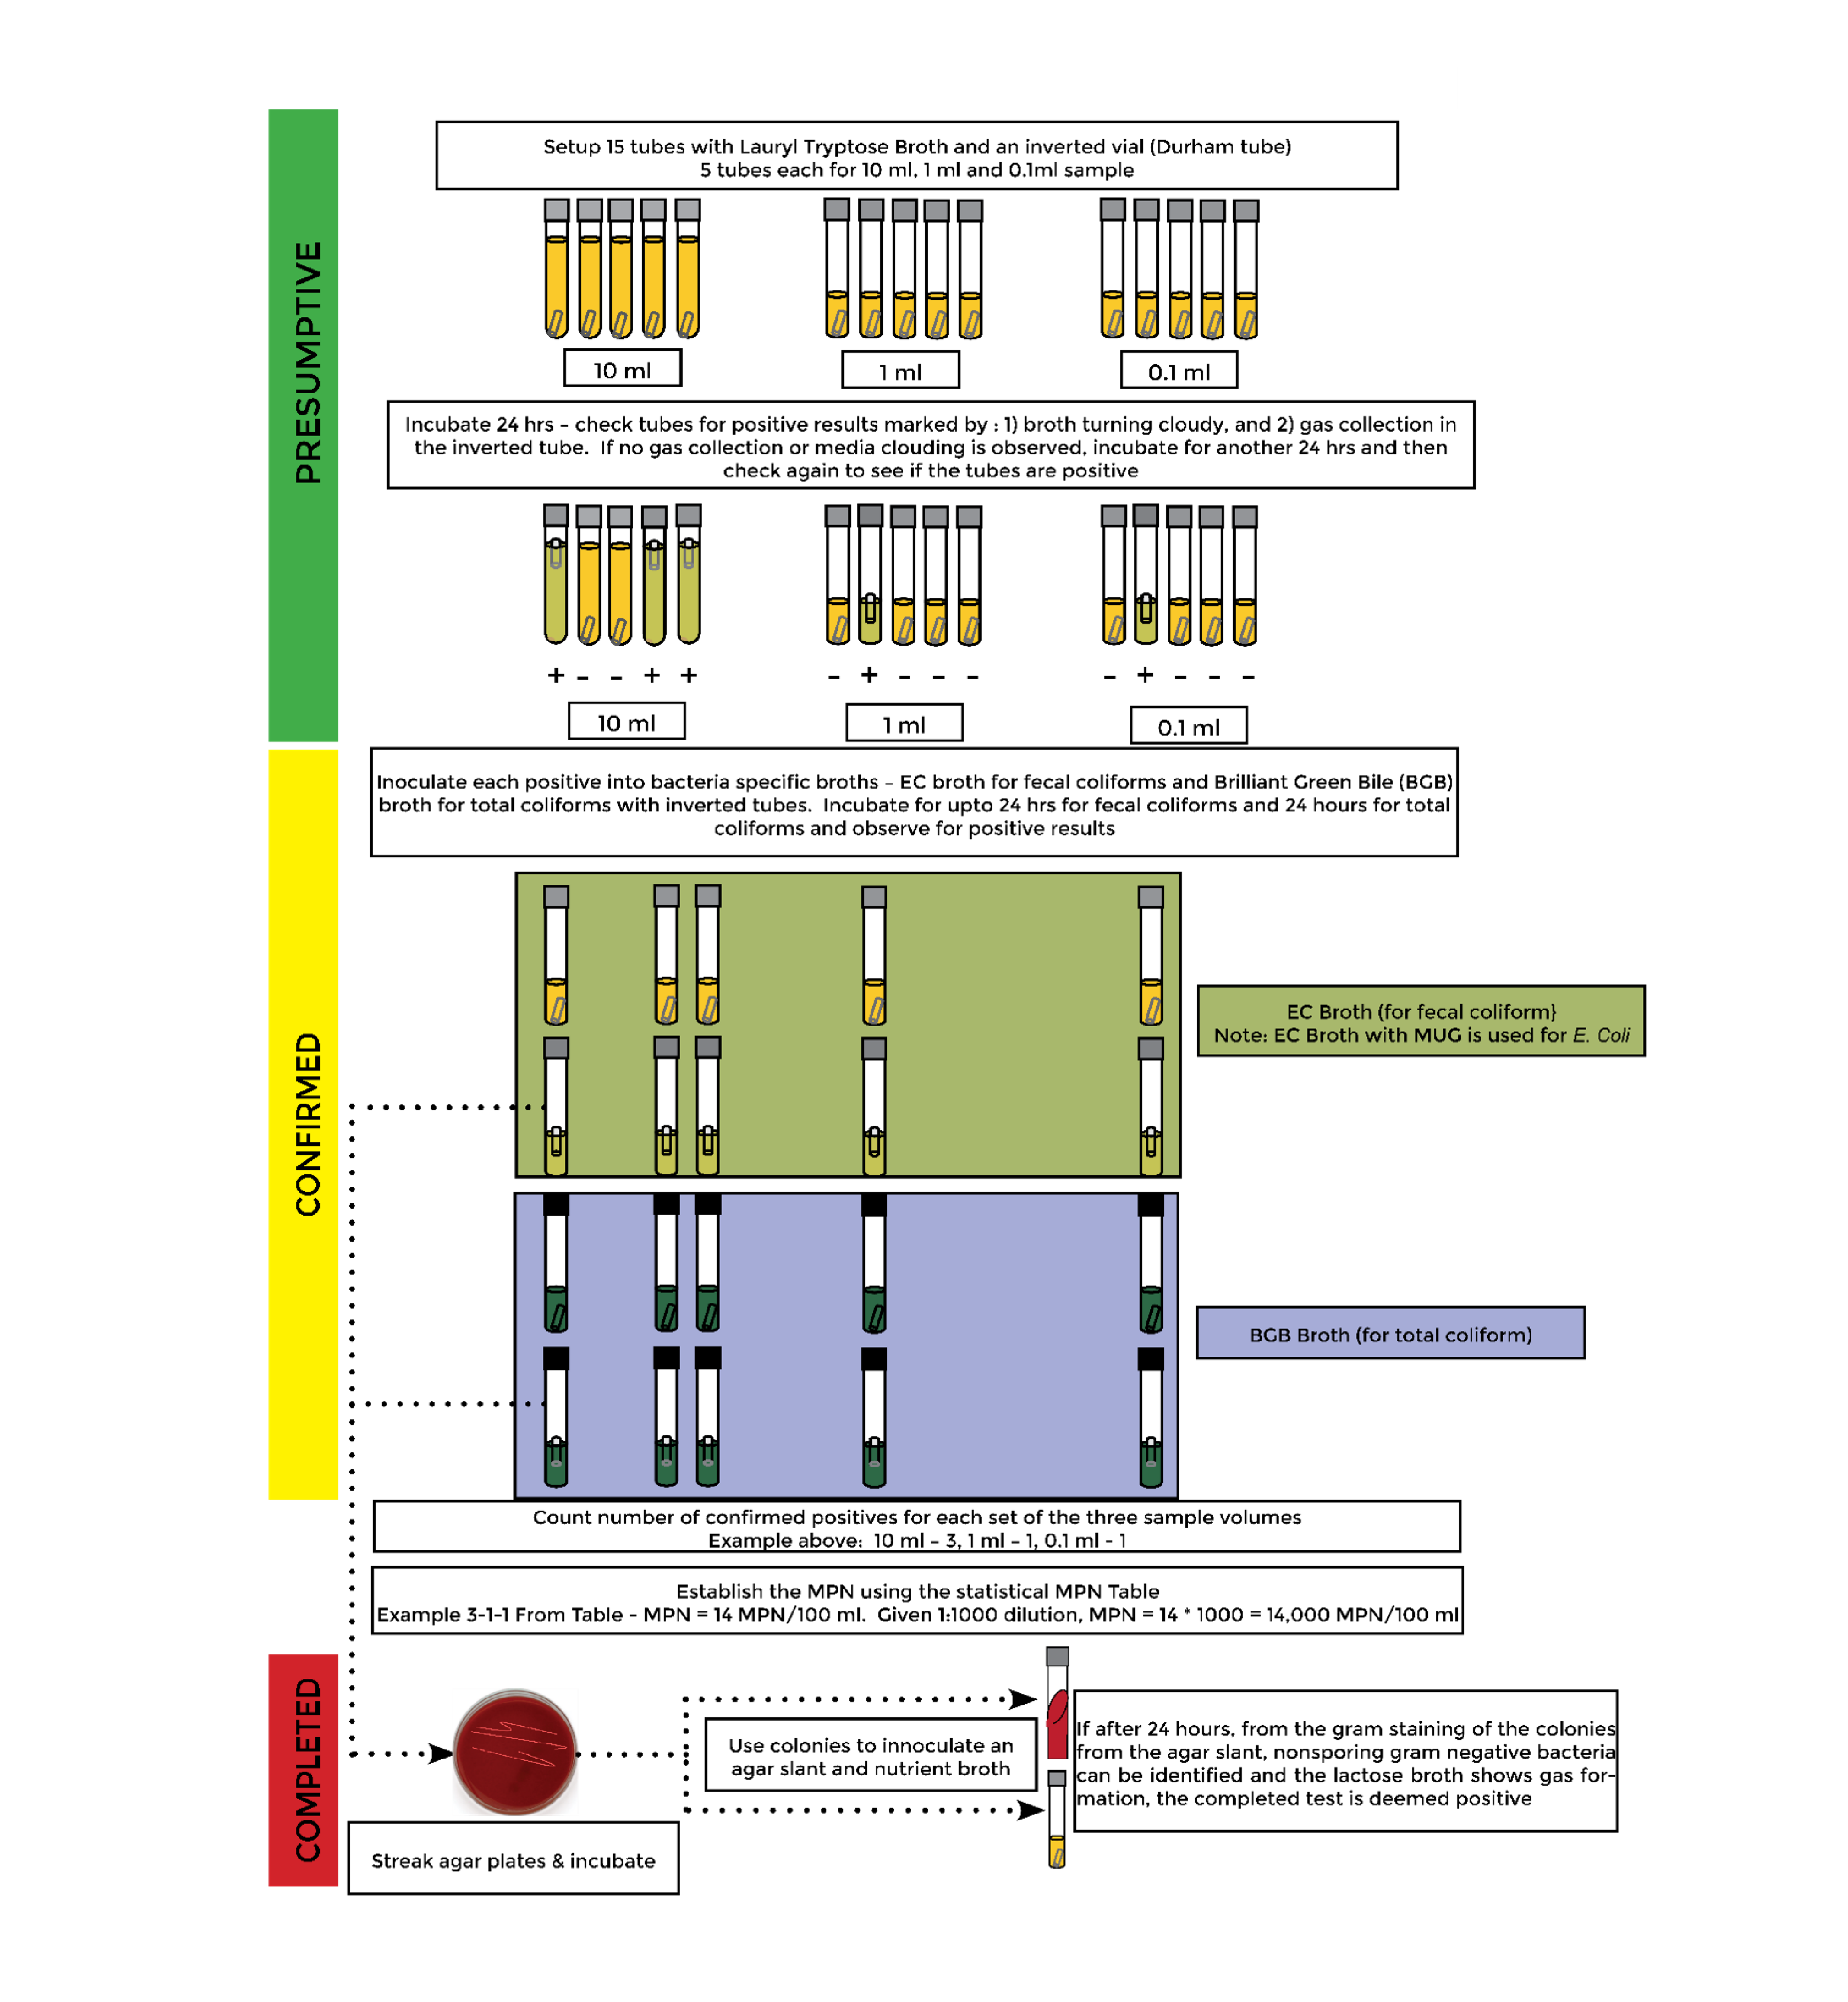
\includepdf[]{WaterMTF.pdf}
%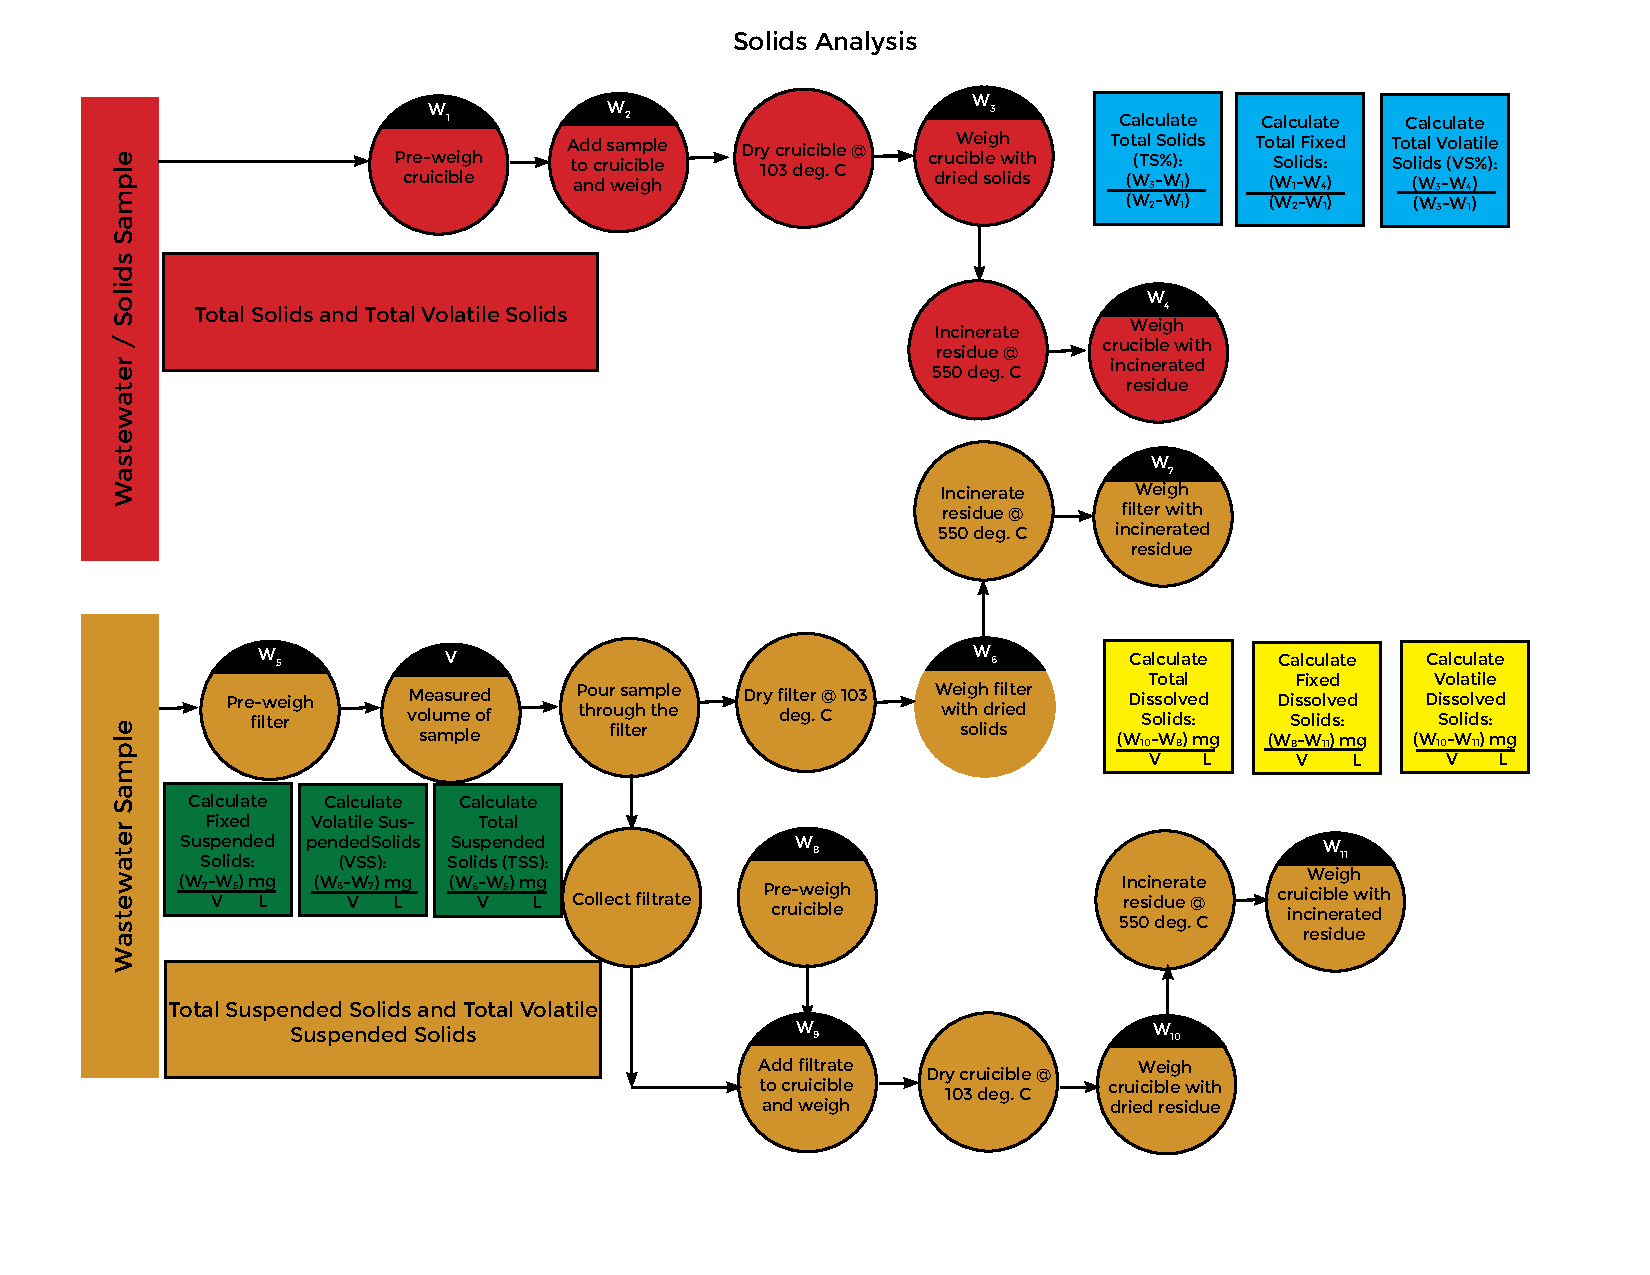
\includegraphics[scale=0.69]{LaboratorySolidsAnalysis4_01.pdf}
% \end{center}
% \end{landscape}
\begin{figure}[H]
\begin{center}
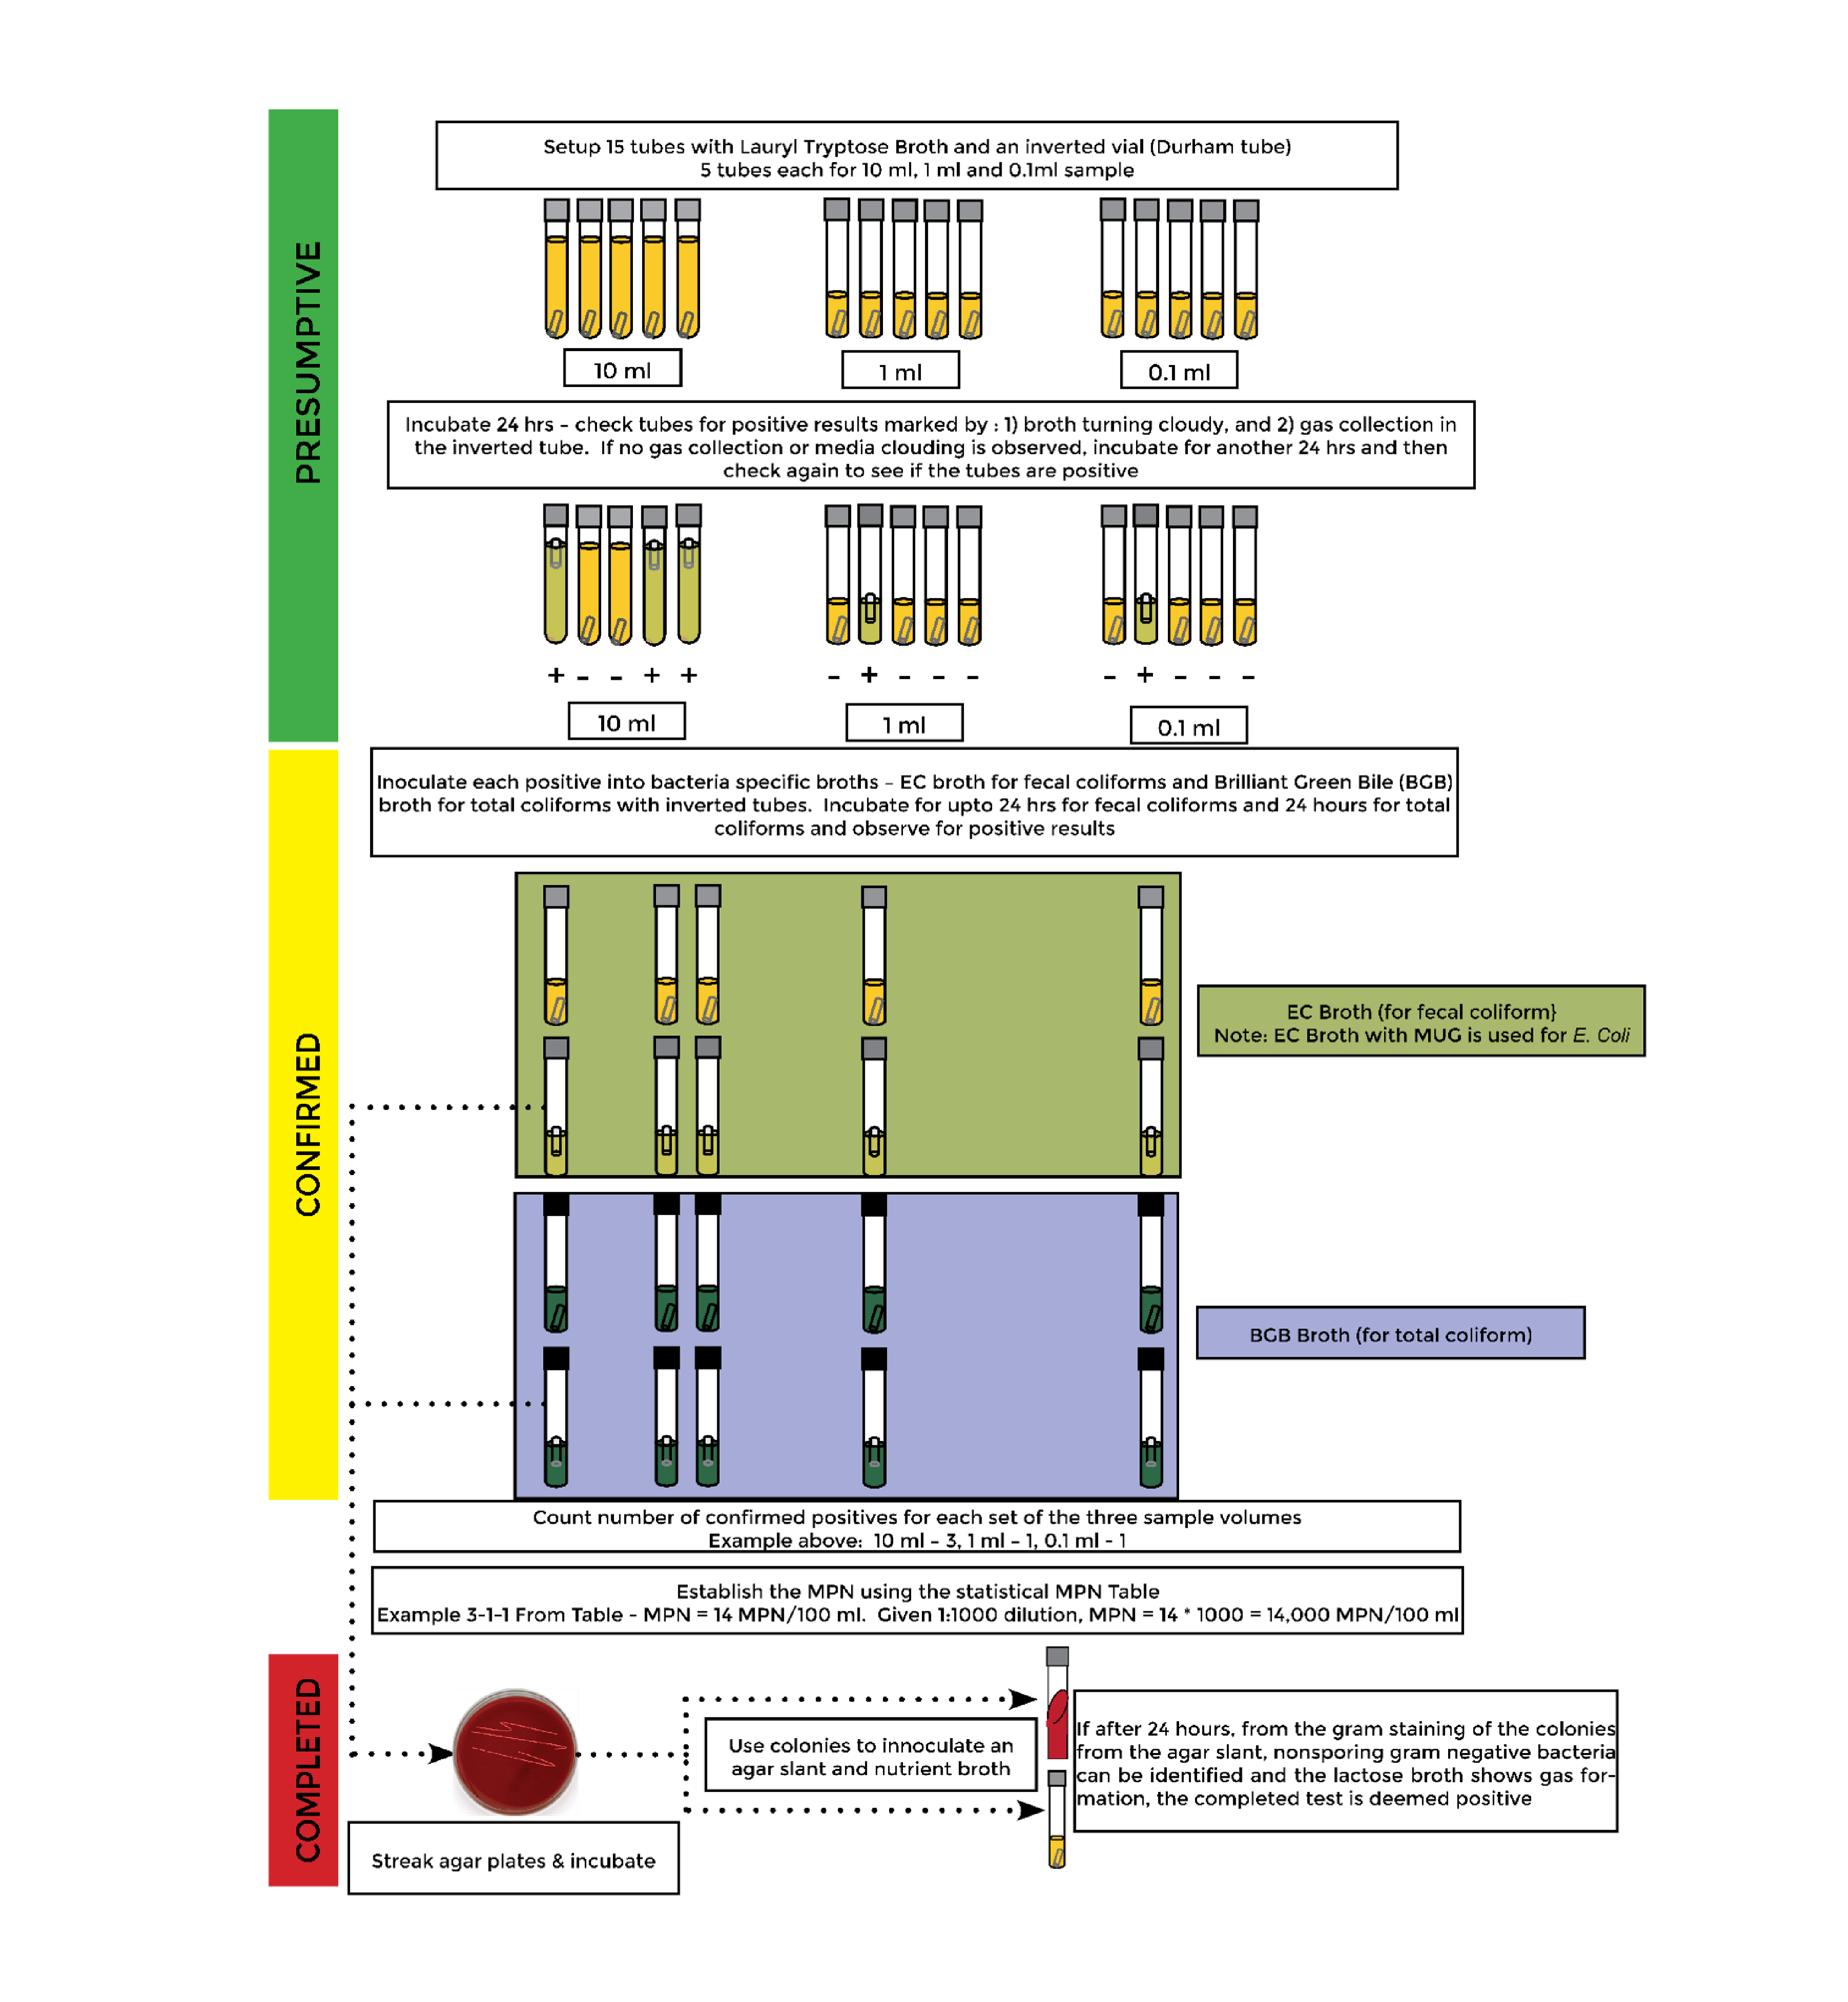
\includegraphics[scale=0.25]{WaterMTF}
\caption{Multiple tube fermentation}
\end{center}
\end{figure}
%\begin{figure}
%\begin{center}
%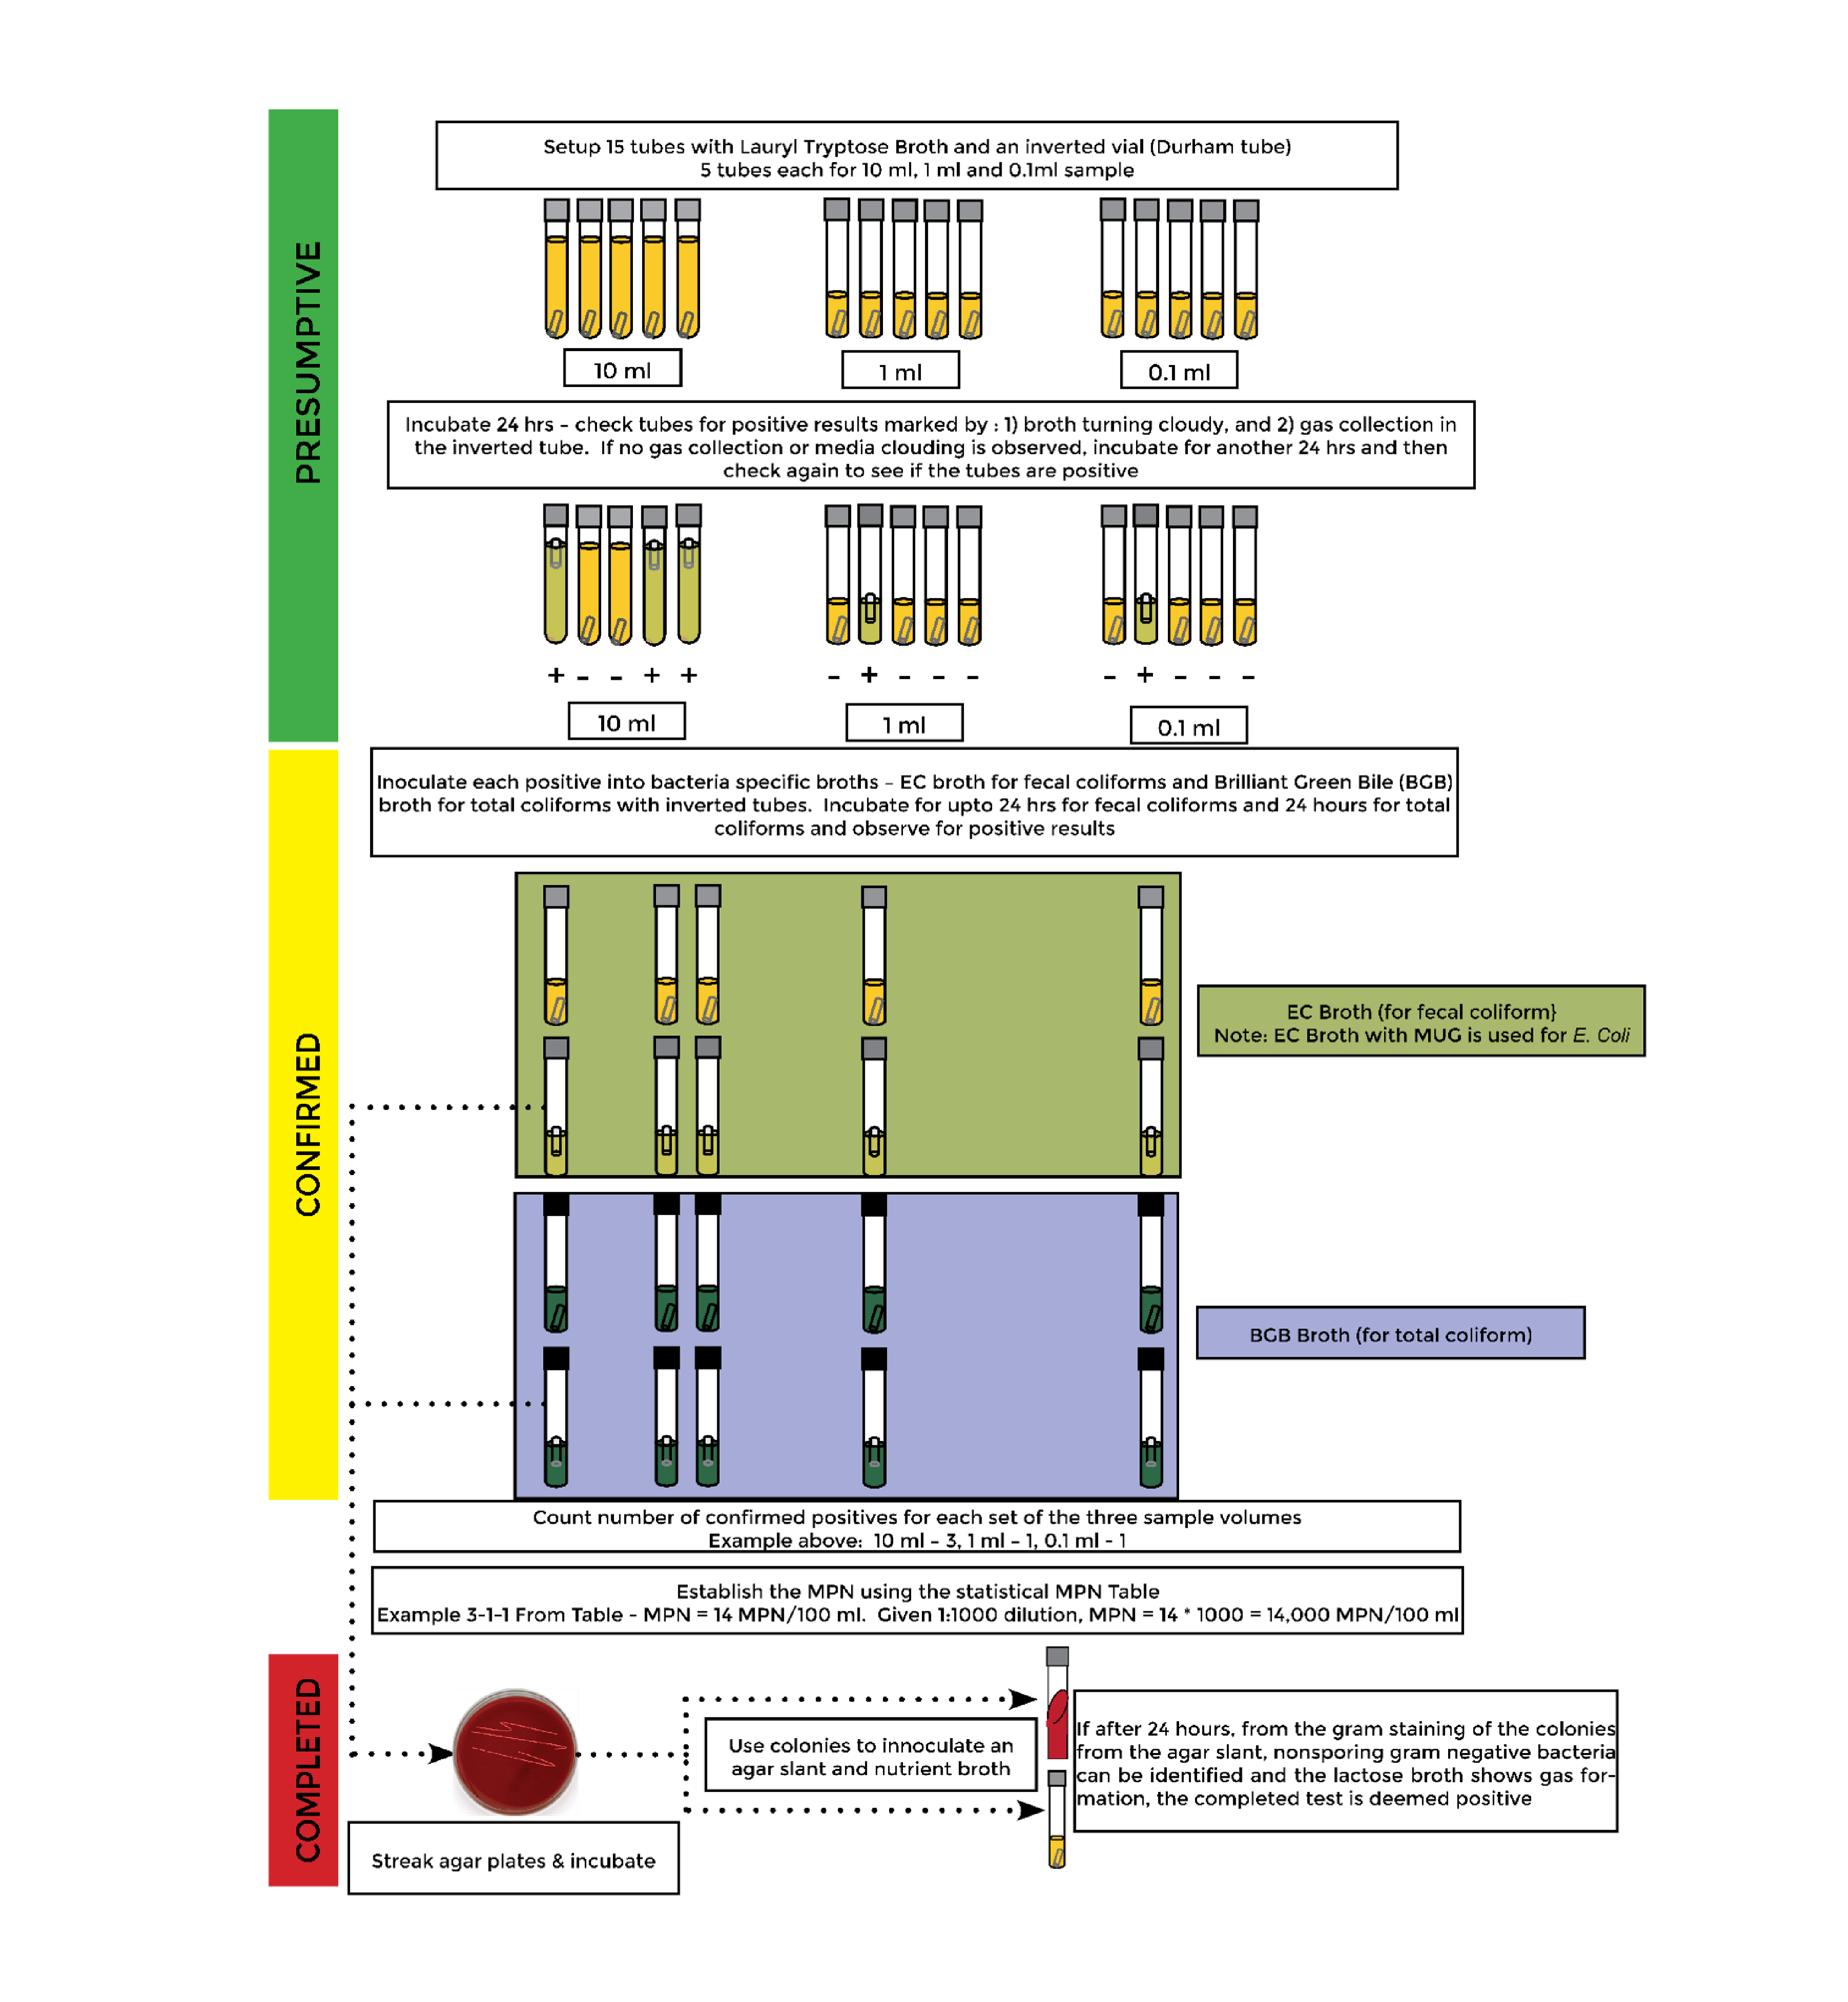
\includegraphics[scale=0.3]{WaterMTF}
%\end{center}
%\end{figure}
\thispagestyle{empty}
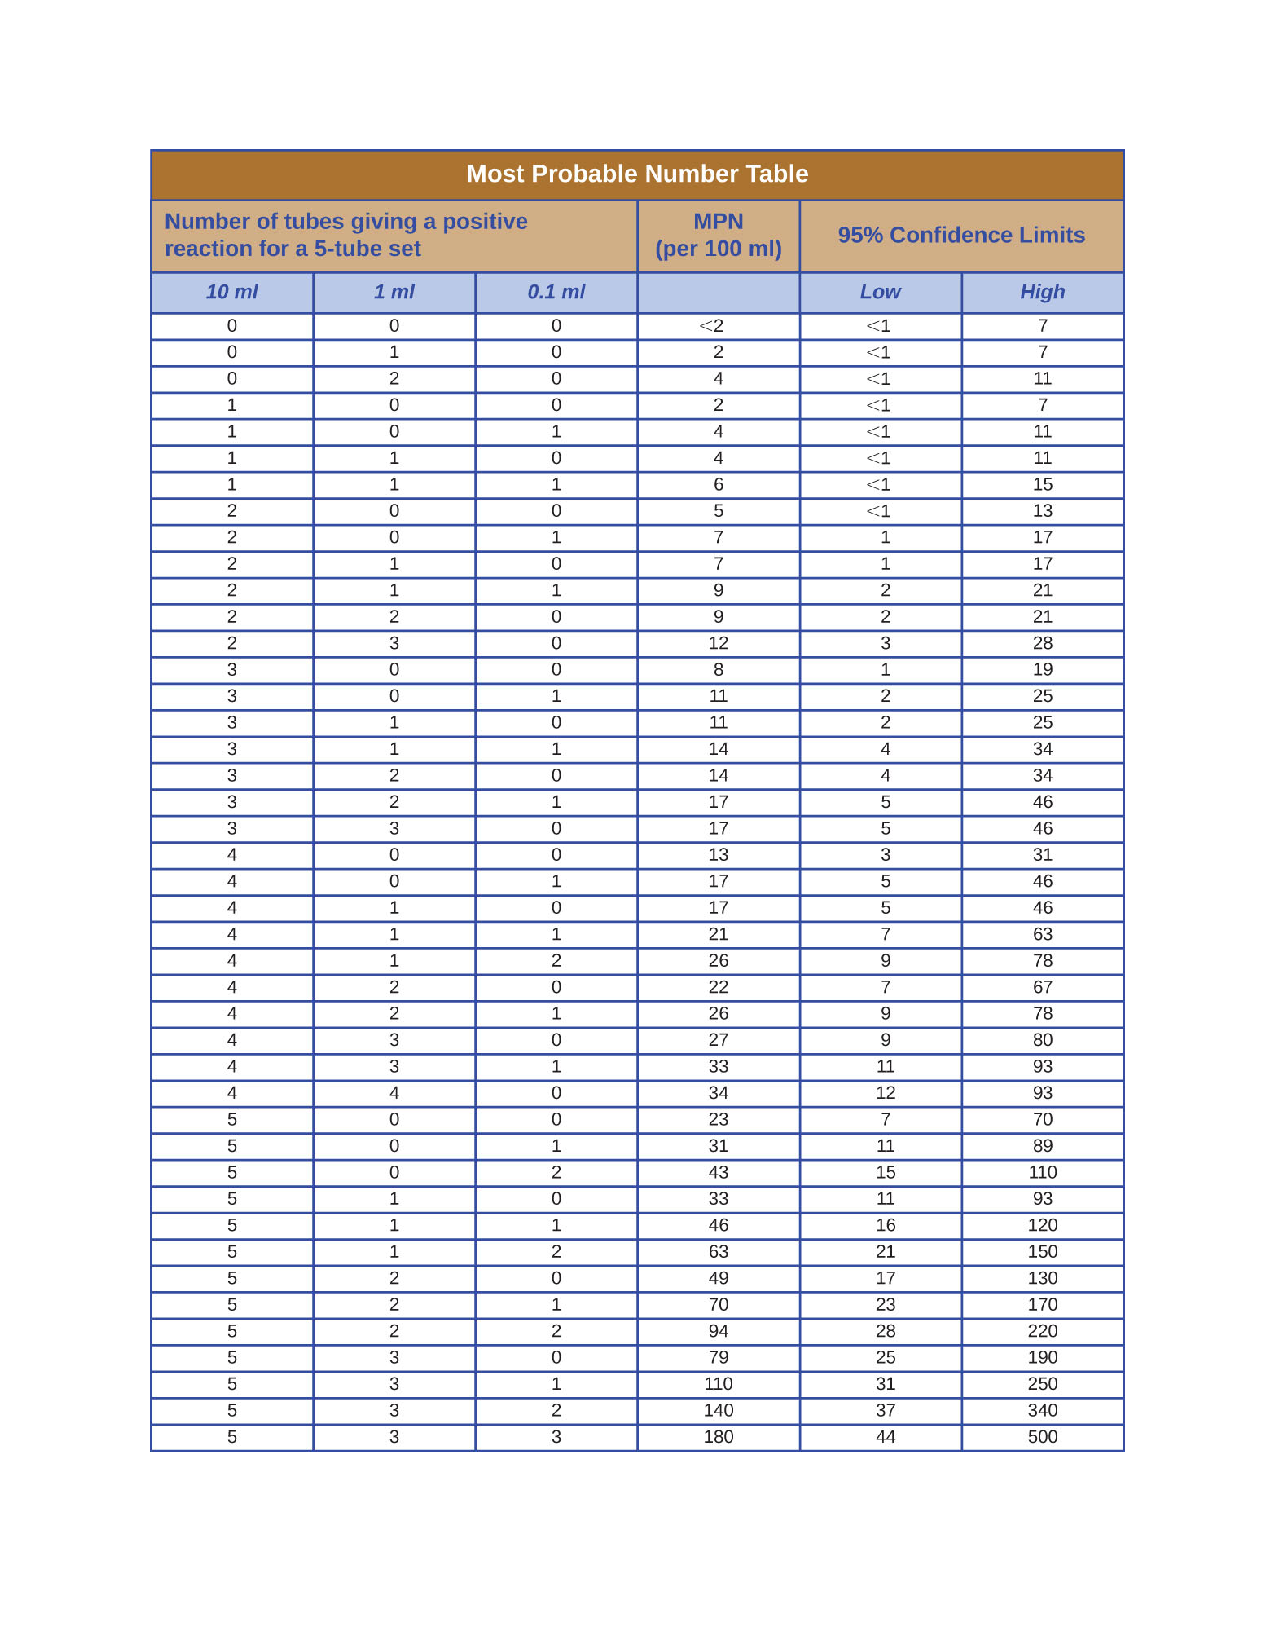
\includepdf[]{MTFTable.pdf}


\newpage

\subsection{Presence - absence (P-A) method}\index{Microbial testing!Presence-absence (P-A) method}
\begin{itemize}
\item Presence - Absence Method below is to assess the presence or absence of bacteria as required by the Revised Total Coliform Rule.
\item The Presence - Absence (P-A) Method for total coliform is based on two premises:
\begin{enumerate}
\item No coliform bacteria should be present in 100 mL of drinking water, and
\item If one viable cell is present it will multiply to give a population of cells that will ferment lactose to produce acid and gas.
\end{enumerate}

\item P-A Method is a simple modification of the multiple tube (MPN) method. P-A broth contains lactose and a pH indicator, which will change from purple to yellow if lactose is fermented and acid is produced. To this P-A broth, the compound \textbf{MUG} has been added. This initially colorless compound can be hydrolyzed by the E. coli to form a compound that fluoresces under long UV light (336 nm). Observing for fluorescence emission using a long-wave (e.g., 365 nm) UV lamp is a sensitive way to confirm the presence of E. coli in water samples.
 
\item The procedure involves addition of 100 ml of sample to 50 ml of sterile P-A broth and then incubating the inoculated broth at 35\degree{C} and inspected after 24 and 48 hours. Upon incubation, a positive result is indicated by the formation of a distinct yellow coloration of the media and/or gas formation which is indicated by foaming of the media upon gentle shaking of the bottle. 

\item Besides the P-A broth, the Colilert test enzymes (used in the above Quanti-Tray test) can be used to test for the Presence-Absence of coliforms.  The colilert enzyme is added to 100 ml water sample in a sterile, non-fluorescing vessel and incubated at 35\degree{C} for 24 h. The results are read at 24 h (before 28 h) and compared against the comparator. If no yellow color, the test is negative, If the sample has a yellow color equal to or greater than the comparator, the presence of total coliforms is confirmed. If yellow, check for blue fluorescence by placing a 6W, 365 nm UV light within 5 inches of the sample. If blue fluorescence is greater or equal to the fluorescence of the comparator the presence of E. coli is confirmed. 
\end{itemize}

\subsection{Heterotrophic plate count (HPC) }\index{Microbial testing!Heterotrophic plate count (HPC)}
\begin{itemize}
\item HPC test - also known as Standard Plate Count is used to measure the overall bacteriological quality of drinking water.
\item  It measures colony formation of heterotrophic bacteria present on culture media. HPC testing indicates the culturable organisms present, which could be as low as 1\% of the total bacteria present. 
\item Heterotrophs are a group of microorganisms including bacteria, molds and yeasts, that use organic carbon sources to grow and can be found in all types of water. Majority of bacteria found in drinking water systems are considered heterotrophs.
\item As all heterotrophic organisms are not pathogens and all pathogens are not heterotrophic, HPC results are not an indicator of water safety.
\item There is no maximum acceptable concentration of HPC in drinking water. However, increases in HPC concentrations above baseline levels are considered undesirable.

\item High HPC counts indicate ideal conditions for bacterial regrowth and should be corrected. Bacterial regrowth can lead to pipe corrosion, encourage slime growth, increase the need for disinfectants, cause foul-tasting water, and harbor secondary respiratory pathogens (ex. Legionella). Thus, HPC can be used as a marker for the underlying causes of some aesthetic problems

\item Methods used for routine testing of heterotrophic bacteria are
\begin{enumerate}
\item Pour plate method: \index{Microbial testing!Heterotrophic plate count (HPC)!Pour plate method}In this method, the liquid sample is poured into the petri dish before the solidification of the agar medium. After solidification, colonies grow both inside and on the surface of the medium.
\item Spread plate method \index{Microbial testing!Heterotrophic plate count (HPC)!Spread plate method}: Here the water sample is spread evenly over the surface of an agar plate medium.  A successful spread plate will have a countable number of isolated bacterial colonies evenly distributed on the plate.
\item Membrane filtration method \index{Microbial testing!Heterotrophic plate count (HPC)!Membrane filtration method}: This test uses a membrane filter is used to capture the bacteria as the water sample is filtered through it.  The filter is placed on an absorbent pad (in a petridish) saturated with a culture medium suitable for heterotrophe growth.
\end{enumerate}

\end{itemize}

\subsection{Other coliform quantification tests}
\ul{Membrane Filtration Method}\index{Microbial testing!Membrane filtration}
Membrane filtration (\textbf{MF}) is a faster way to estimate bacterial populations in water.  In this method, an appropriate sample volume is passed through a membrane filter with a pore size small enough (0.45 micron) to retain the bacteria present. The filter is placed on an absorbent pad (in a petri dish) saturated with a culture medium that is selective for coliform growth. The petri dish containing the filter and pad is incubated, upside down, for 24 hours at the appropriate temperature. After incubation, the colonies that have grown are identified and counted using a low power microscope. A MUG medium is used for E- Coli.  If E. Coli is present, it will make the MUG fluorescent when viewed in UV light. 


\begin{figure}[!htb]
    \centering
       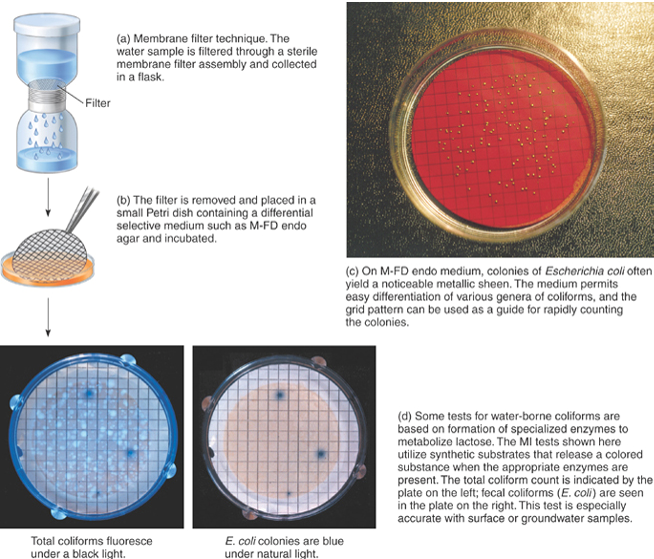
\includegraphics[width=\linewidth]{LaboratoryMembraneFiltration}
        \caption{Multiple tube fermentation}
    \end{figure}
    
\ul{Quanti-trays tests}\index{Microbial testing!Quanti-trays tests}

This test used for the detection and quantification of specific microorganisms is being used increasingly mainly because it is a quicker test than the MTF.  Colilert and Enterolert \index{Microbial testing!Colilert} are the quanti tray based tests for E. Coli and Enterococcus.  This method involve the use of specific enzymes and overcomes the drawbacks of the MTF which include false positives and negatives due to the more generic nature of the media used.
\begin{figure}[!htb]
    \centering
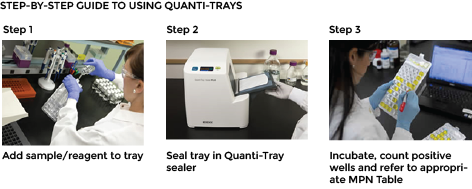
\includegraphics[width=\linewidth]{LaboratoryQuantiTray}
\caption{Quanti-trays test}
\end{figure}

\section{Sampling}\index{Sampling}

		\begin{itemize}
			\item Field or laboratory measurement of a certain parameter is critical in water treatment and distribution operations to obtain information about characteristics of water.
			\item A sample is a small part of the whole representing the whole.  Thus, a sample needs to be such that it truly represents the entire population – which could be either a treatment process stream or what is provided to the end user.
			\item As not all water is analyzed, a sample obtained for analysis must “represent” varying:
			\begin{itemize}
			\item Locations:  Locations should be representative of the majority of their portion of the Distribution System. Unusual locations should be avoided, as they are not indicative of the system as a whole.  Such locations are often monitored, but not as part of the routine plan.

			\item Time periods: Time period samples include:
			\begin{itemize}
			\item Grab: \index{Sampling!Grab} Sample taken in a single moment of time.
			\item Composite: \index{Sampling!Composite} Several portions collected over time and/or space.
			\item Continuous

			\end{itemize}
		\end{itemize}
		\end{itemize}


\subsection{Sampling methods}\index{Sampling!Sampling methods}

\subsubsection{Grab samples}\index{Sampling!Grab samples}
				\begin{itemize}
					\item A grab sample is a sample collected at a specific spot at a site over a short period of time.  
					\item Grab sampling allows for instantaneous analysis of parameters such as pH, dissolved oxygen, chlorine residual, temperature and other parameters which change rapidly with time.
					\item A grab sample represents a snapshot of space and time of a process stream.
					\end{itemize}

\subsubsection{Composite Samples}\index{Sampling!Composite Samples}
				\begin{itemize}
					\item A composite sample is a collection of discrete samples are combined over a certain period or space and therefore represent the average performance of a treatment plant or a process during the collection period.\\  
					\item Composite sampling can be either based on:
					      
					      1. constant time interval (time-proportioned sampling)\index{Sampling!Composite!time-proportioned sampling}\\
					      2. constant volume interval (flow-proportioned sampling), \index{Sampling!Composite!flow-proportioned sampling}and\\
					      3. treatment process space - includes samples taken at different depths \index{Sampling!Composite!depth sampling}\\
					      
					\item Composite samples are typically collected using automated samplers which can be programmed to collect samples at preset time intervals – for time proportional sampling.
					\item Time and space composite samples are collected by adding equal volumes of samples collected from different times or locations.  
					\item Flow proportional composite samples comprise of volume of each subsample based on flow.\\  
				\end{itemize}
	\begin{figure}			
			\begin{center}
				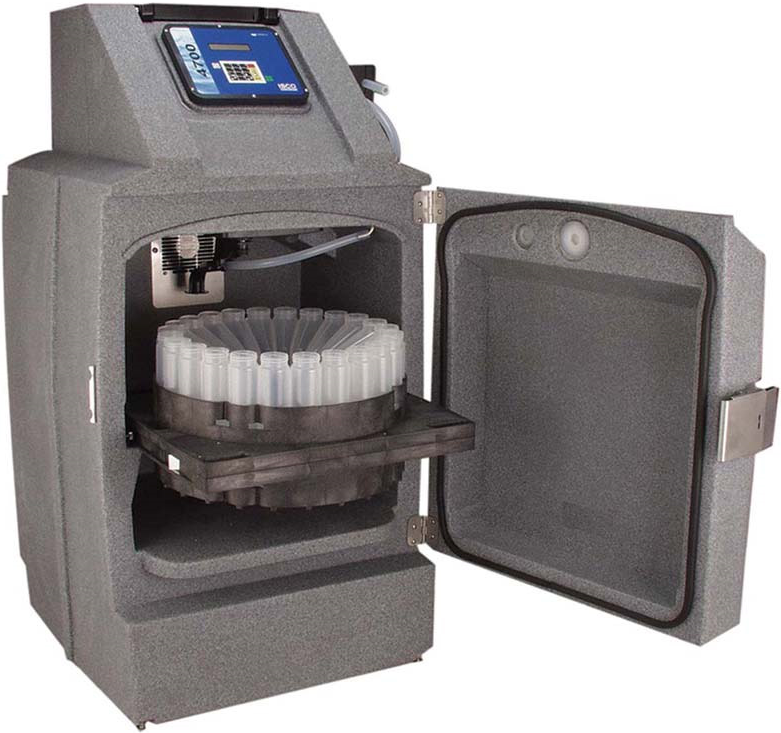
\includegraphics[scale=0.2]{Autosampler} \hspace{2cm} 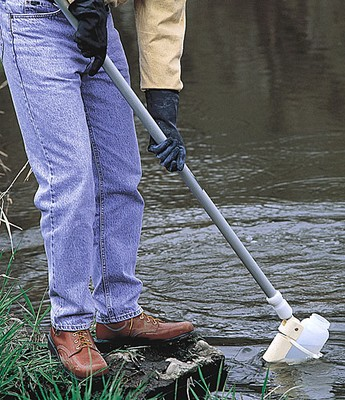
\includegraphics[scale=0.37]{Grabsampler}\\
			\end{center}
			\hspace{2.3cm} Automated Sampler \hspace{2.0cm} \parbox{\textwidth}{Grab Sampling Using a Long Handle Dipper}\\
\end{figure}
\subsection{Sampling precautions and protocols}\index{Sampling!Precautions and protocols}
			\begin{itemize}
				\item Samples should represent the major portion of the process or the process stream and should be taken from places where the mixing is thorough, avoiding dead spots and areas of heavier or lighter loadings. 
				\item The collected sample is invariably exposed to conditions very different from the original source and is subject to change due to chemical and microbiological activity.  
				\item Thus, in order to ensure integrity of sample, sample preservation techniques specific to the analysis to be performed is needed.  
				      \begin{itemize}
				      	\item The preservation technique should not only allow for stabilizing the parameter to be analyzed, it should also not interfere with the analyses.  
				      	\item The common preservation techniques involve use of proper containers, temperature control, addition of chemical preservatives, and observance of the recommended maximum sample holding time.
				      \end{itemize}
				      \item Samples cannot be held indefinitely prior to lab analysis
\item  Laboratories used for testing must be approved by Environmental Laboratory Accreditation Program {ELAP} \index{Environmental Laboratory Accreditation Program (ELAP)} and must use Standard Methods.
\item Chain-of-custody \index{Chain-of-custody}ensures sample integrity from collection to data reporting Important for sample control when litigation is involved Must be under a person’s physical possession, within sight, or secured in a restricted area Receipt and logging of sample at lab Complete documentation from collection to report
\item Sample Containers:
\begin{itemize}
\item Typically plastic or glass
\item Use proper material for analysis
\item Use glass for all organic and odor analyses
\item Use plastic for metals
\item Bacteriological sample containers must be sterile
\end{itemize}
\end{itemize}

\subsection{Microbial sampling}\index{Sampling!Microbial sampling}
\begin{itemize}
\item Always collected as a grab.
\item The sample is obtained from a steady, pencil-width stream from a cold water fixture, only after it has been in a wide open setting and  water to run a minimum of five minutes to flush out the bacteria from the surface. 
\item A clean, sterile borosilicate glass or plastic bottle containing sodium thiosulfate is used. Sodium thiosulfate is added to remove residual chlorine which will kill the microorganisms during transit. If the sample is not preserved or maintained under proper conditions until the test is conducted in the laboratory, the test would provide erroneous results
\item Samples must be refrigerated if they cannot be analyzed within 1 hour of collection
\item Samples must be handled with care to prevent contamination and adverse conditions such as prolonged exposure to direct sunlight
\item Maximum holding time for state or federal permit reporting purposes is 6 hours
\item Number of samples collected depends on number of customers served/and is according to the approved sample siting plan.
\item The volume for coliform compliance sample must be at least 100ml and no more than 120ml. 
\item Sealed and sterilized sampling bottles - typically, 120 ml with 100 ml marked to provide space for air is used.
\item Sodium thiosulfate or some other de-chlorinator \index{Chlorine disinfection!Dechlorination}is pre-added to the sampling bottle. A dechlorinator is critical to ensure any chlorine residual is removed from the sample collected.
\item The faucet is opened to obtain a continuous flow of the size of a pencil, the faucet should not be opened under a strong flow as  that could potentially dislodge loose particles/slime growth in the mains.
\item When the cap is opened to collect the sample, care needs to be taken to ensure the cap is not contaminated.
\item Fill the bottle to the marked fill-line leaving an air gap - do not overfill.
\item The capped bottle should be placed in an iced container and transported to the laboratory as soon as possible.
\item Follow chain-of-custody \index{Chain-of-custody}and send the bottles to the lab with paperwork.
\item In the laboratory, the samples must be kept at 4\degree{C} or 39\degree{F} and must be analyzed preferably within 8 hours and never to exceeding 24 hours.
\item The analytical results shall be reported in terms of the presence or absence of total coliforms and E. coli, in the sample, whichever is appropriate.
\item Monthly sampling results must be submitted to the regulatory agency per established scheduled.
\item Records of bacteriological sampling must be kept for five years \index{Bacteriological sampling records}.
\item Repeat sampling:  If the result is positive a minimum three samples need to be taken, one from the original point, one up-stream and one from downstream of the original sample collection site within 24 hours after the result notification from the laboratory.
\item False positive means that the sample when tested is found to be contaminated but
actually the water is safe.
\item False negative means samples are found to be safe; even though the water is
- unsafe to drink. This can lead to outbreak of diseases and cause customers to lose confidence in their drinking water supplier. This harms the customer. \index{False negative/positive}
\end{itemize}
\newpage
\subsection{Summary of sampling requirements}\index{Sampling!Summary of sampling requirements}\index{Sampling!Preservative}\index{Sampling!Holding time}
\begin{table}[h!]
\begin{tabular}{|p{4cm}|p{3cm}|p{4cm}|p{3cm}|}
\hline
\multicolumn{1}{|c|}{\textbf{Parameter}}                                                   & \multicolumn{1}{c|}{\textbf{Container}}                                            & \multicolumn{1}{c|}{\textbf{Preservative}}                                                                                                                   & \multicolumn{1}{c|}{\textbf{Holding Time}}                          \\ \hline
\begin{tabular}[c]{@{}l@{}}Coliform, total or fecal,\\      in chlorinated water\end{tabular} & \begin{tabular}[c]{@{}l@{}}Sterile container    w/\\      thiosulfate\end{tabular} & Cool   to \textless{}10 °C.  Do not freeze                                                                                                                    & 8   hrs for source water compliance and 30 hours for drinking water \\ \hline
Giardia and   Cryptosporidium                                                              & 10   L plastic container                                                           & Cool   to \textless{}10  °C .  Do not freeze                                                                                                                    & 96   hours                                                          \\ \hline
Alkalinity, turbidity, solids                                                             , fluoride & Plastic or Glass                                                                   & Cool   to \textless{} 4 °C                                                                                                                                             & Method   dependent                                                  \\ \hline
Metals, general                                                                            & Plastic or Glass, Rinsed w/ 1:1 HNO$_3$                                               & Nitric   acid to pH \textless 2                                                                                                                              & 6 Months                                                            \\ \hline
Hardness                                                                           & Plastic or Glass                                                                   & Nitric   acid to pH \textless 2                                                                                                                              & 6 Months                                                            \\ \hline
pH                                                                                         & Plastic or Glass                                                                   & None                                                                                                                                                         & Analyze in 15 min                                                    \\ \hline
Nitrogen and   phosphorous compounds                                                       & Plastic or Glass                                                                   & Sulfuric acid to   pH\textless{}2                                                                                                                            & 28 days                                                             \\ \hline
VOCs, TTHMs                                                                                & Glass bottle                                                                       & Sodium thiosulfate or   ascorbic acid if sample is chlorinated and hydrochloric acid (HCl) to pH \textless 2  and cool to  \textless 4 °C  but do not freeze & 14 days                                                             \\ \hline
\end{tabular}
\caption{Summary of sampling requirements for key parameters}\index{Sampling!Summary of requirements}
\end{table}





